\documentclass[11pt,a4paper,oneside,table,xcdraw]{report}

% CREATED BY DAVID FRISK, 2015


% BASIC SETTINGS
\usepackage{url}
\usepackage{lastpage}								% Get the number of pages
\usepackage{moreverb}								% List settings
\usepackage{textcomp}								% Fonts, symbols etc.
\usepackage{lmodern}								% Latin modern font
\usepackage{helvet}									% Enables font switching
\usepackage[T1]{fontenc}							% Output settings
\usepackage[english]{babel}							% Language settings
\usepackage[utf8]{inputenc}							% Input settings
\usepackage[table]{xcolor} 							% Table colors
\definecolor{light-gray}{gray}{0.96}			% Defining a very light gray for a table

\usepackage{amsmath}								% Mathematical expressions (American mathematical society)
\usepackage{amssymb}								% Mathematical symbols (American mathematical society)
\usepackage{graphicx}								% Figures
\usepackage{subfig}									% Enables subfigures
\numberwithin{equation}{chapter}					% Numbering order for equations
\numberwithin{figure}{chapter}						% Numbering order for figures
\numberwithin{table}{chapter}						% Numbering order for tables
\usepackage{listings}								% Enables source code listings
\usepackage{xparse}								% Enables in-line code
\NewDocumentCommand{\codeword}{v}{ % Enables in-line code
	\texttt{\textcolor{blue}{#1}}
}
\usepackage{chemfig}								% Chemical structures
\usepackage[top=3cm, bottom=3cm,
			inner=3cm, outer=3cm]{geometry}			% Page margin lengths			
\usepackage{eso-pic}								% Create cover page background
\newcommand{\backgroundpic}[3]{
	\put(#1,#2){
	\parbox[b][\paperheight]{\paperwidth}{
	\centering
	\includegraphics[width=\paperwidth,height=\paperheight,keepaspectratio]{#3}}}}
\usepackage{float} 									% Enables object position enforcement using [H]
\usepackage{parskip}								% Enables vertical spaces correctly 
\usepackage{minted}
%Code highlighting and formatting
\usepackage{dirtree}
\usepackage{epigraph}
%Appendix
\usepackage[toc,page]{appendix}
\usepackage{wrapfig}
\usepackage{caption}
% OPTIONAL SETTINGS (DELETE OR COMMENT TO SUPRESS)

% Disable automatic indentation (equal to using \noindent)
\setlength{\parindent}{0cm}                         


% Caption settings (aligned left with bold name)
% \usepackage[labelfont=bf, textfont=normal,
%			justification=justified,
%			singlelinecheck=false]{caption} 		

		  	
% Activate clickable links in table of contents  	
\usepackage{hyperref}								
\hypersetup{colorlinks, citecolor=black,
   		 	filecolor=black, linkcolor=black,
    		urlcolor=black}


% Define the number of section levels to be included in the t.o.c. and numbered	(3 is default)	
\setcounter{tocdepth}{5}							
\setcounter{secnumdepth}{5}	


% Chapter title settings
\usepackage{titlesec}		
\titleformat{\chapter}[display]
  {\Huge\bfseries\filcenter}
  {{\fontsize{35pt}{1em}\vspace{-4.2ex}\selectfont \textnormal{\thechapter}}}{1ex}{}[]


% Header and footer settings (Select TWOSIDE or ONESIDE layout below)
\usepackage{fancyhdr}
\pagestyle{fancy}
\fancypagestyle{plain}{}
\lhead{}
\rhead{}
\renewcommand{\chaptermark}[1]{\markboth{\thechapter.\space#1}{}}


\fancyhf{}
\fancyhead[L]{Daniel Kartin\\Marcus Skytt\\Rasmus Kruuse}
\fancyhead[C]{MED3\\AAU CPH}
\fancyhead[R]{Nicolai Kloch Lorits\\Simone Danielsen\\Jens Jákup Gaardbo}
\fancyfoot[C]{\thepage}

\usepackage[final]{pdfpages}
\usepackage{verbatim}
\usepackage{lipsum}
\usepackage{multicol}
% Enable To-do notes
\usepackage[textsize=tiny]{todonotes}   % Include the option "disable" to hide all notes
\setlength{\marginparwidth}{2.5cm} 

\usepackage{tikz}
\usetikzlibrary{mindmap,trees}
\usepackage{nameref}

% Supress warning from Texmaker about headheight
\setlength{\headheight}{30pt}		

\newcommand{\HRule}{\rule{\linewidth}{0.5mm}}

\usepackage[normalem]{ulem}
\useunder{\uline}{\ul}{}


\usepackage[square,numbers,sort&compress]{natbib}
\bibliographystyle{unsrtnat}

\usepackage{tocbibind}

\usepackage{tikz}
\usepackage{pgf-pie}
\usepackage{pgfplots}
\pgfplotsset{width=12cm,compat=1.11}
\pgfplotsset{
	cycle list={red\\blue\\},
}
\usepgfplotslibrary{statistics}






\begin{document} 

	
% COVER PAGE, TITLE PAGE AND IMPRINT PAGE
\pagenumbering{roman}					% Roman numbering (starting with i (one)) until first main chapter
\begin{titlepage}
\newgeometry{top=3cm, bottom=3cm,
			left=2.25 cm, right=2.25cm}	% Temporarily change margins		
			
% Cover page background 
\AddToShipoutPicture*{\backgroundpic{-4}{56.7}{figure/Frontpage/frontpage-aau.pdf}}
\addtolength{\voffset}{2cm}

% Cover picture 		
\begin{figure}[H]
\centering
\vspace{2cm}	% Adjust vertical spacing here
\includegraphics[width=0.99\linewidth]{figure/Frontpage/gardenposterCropped.png}
\end{figure}

% Cover text
\mbox{}
\vfill
\renewcommand{\familydefault}{\sfdefault} \normalfont % Set cover page font
\HRule\\[0.1cm]
\textbf{{\small Medialogy P3\\ {\Huge Garden box}}} \hspace{0.15cm} {\Huge \color{gray}-} \hspace{0,15cm}{\Huge \color{gray}plan it, plant it}\\
\HRule\smallskip{}
\begin{multicols}{2}
{\Large Daniel Kartin\\Jens Jákup Gaardbo\\Marcus Skytt\\Nicolai Kloch Lorits\\Rasmus Isager Kruuse\\Simone Danielsen\columnbreak}\\
\setlength{\parskip}{2.4cm}
{\Large{\textbf{Supervisor}\\Daniel Overholt\\dano@create.aau.dk}}\medskip\\
\href{https://github.com/CakeFTW/unityOpencvPlugin}{\color{blue}Plugin repository}\\
\href{https://youtu.be/wmZ-fhU4JIE}{\color{blue}Project video}\medskip
\\\small AAU CPH - 
MED3 \\
Group 307\\
\end{multicols}
\today
\renewcommand{\familydefault}{\rmdefault} \normalfont % Reset standard font
\end{titlepage}





\thispagestyle{plain} % Suppress header 
\setlength{\parskip}{0pt plus 1.0pt}
\includepdf[pages=-]{include/frontmatter/Page_0.pdf}


% INDHOLDSFORTEGNELSE
\tableofcontents

\todo{generelt synes jeg det er rigtig godt, har dog nogle generelle ønsker: 1) HUSK AT LAVE REFERENCER! der er mange afsnit hvor der ikke er en eneste! og mange steder er der for få. husk for hvert udsagn skal der en reference. - også billeder og citater! 2) har nogle ønsker til lidt omrokeringer - interaction skal være det først underpunkt under lærings afsnittet, og FPSen skal rykkes op under "choice of direction" da det er her vi beslutter hvad der skal så i FPSen)}
 
\newpage

\newpage

\setcounter{page}{1} 					% Arabic page numering (starting at 1(one)) throughout the paper
\pagenumbering{arabic}

% INDLEDNING
\chapter{Introduction}
	Designing a garden can be a time demanding affair. People with a newly built house or garden might hire a landscape architect to take on the design process. As technology evolves, new mediums to demonstrate great garden designs to a client get introduced\cite{landscapeArchitectureDigiTech}. First it was 3D scenes, conveying the design of a garden through a video tour. Now, the next big leap in visualization technology is Virtual Reality\cite{VRS}, and with it comes the ability to show off garden designs to clients in an entirely new way.\\
	
	Some garden architects might find it hard to fully incorporate three dimensional designs into their workflow. The process is time consuming and the software can be difficult to learn, hence only a few actually make use of it. Instead they stick with traditional sketching by hand to communicate their idea to the customers, who risk not being able to fully and accurately envision how the garden will look when it has been completed.\\
	
	In recent years more and more products, such as VR Gardens and Invita Kitchen VR, have been developed that take the three dimensional aspect to another level by incorporating immersive Virtual Reality(VR) into architecture and interior design, which allows a user, wearing a Head Mounted Display(HMD), to step into, and experience, a virtual representation of their future kitchen or garden.\\
	
	For the purposes of this project, the focus will be on the design process of a landscape architect and the quality and speed of the concept visualization during that process. A prototype of an alternative tool for landscape architects which utilizes immersive VR will be presented, evaluated and discussed. A comparison of the prototype and traditional visualization methods, 2D sketches and 3D renderings, will be made with the focal point being the percieved immersiveness.
	
	
	\section{Initial problem statement}
	How can the garden design process be improved by putting the user in a 3D VR environment created from a simple sketch using image processing?
	

% ANALYSE
\chapter{Analysis}
In this analysis, the focus will be on the investigation of the current issues with the fundamentals of musical education in elementary schools.\\
\\
Furthermore, current tools and technological inventions will be investigated to incorporate the similar aspects into a final prototype.

\section{Problem Area}
	To narrow down the subject and get a better understanding of what the problem is and which target group to work with, some initial research had to be made and the study plans for danish elementary schools from grade 1 through 6 was investigated.\\
	
	\subsection{The impact of musical education}
	Several studies have shown that different types of musical engagement in a variety of ways over a lifespan has an impact on several aspects of personal growth and development. As concluded in the article "The power of music: Its impact on the intellectual, social and personal development of children and young people":\\
	
	\begin{quote}
		\textit{"This overview provides a strong case for the benefits of active engagement with music throughout the lifespan"}\cite{powerOfMusic}\label{quote:powerOfMusic}.\\
	\end{quote}
	
	Linguistic abilities and musical training seems to be linked, due to shared brain mechanisms being used to process music and language. Precision in the perception of speech related contrasts, in pitch patterns and other distinctive speech elements have been reported to be associated with musical ability\cite{languageSkills}.\\
	
	A study focused on literary skills showed that a group of second grade students(n = 47) taking piano lessons over a 3-year period had significantly better vocabulary and verbal abilities than a group of control students(n = 57) that did not receive music lessons\cite{vocabularySkills}.\\
	
	Some aspects of mathematical skills have also been shown to be improved by musical training. For example the subdivision process required to read and play from music scores in order to play and keep a rhythm\cite{powerOfMusic}.\\
	
	Other abilities have also been reported to be affected by musical training such as creativity, social and personal development, physical development, health and wellbeing\cite{powerOfMusic}.\\
	
	According to the article \textit{Interactive music video games and children's musical development} there are 5 basic music elements that should be learned in order to get a good understanding and appreciation of music\cite[p.~99]{interactiveMusicVideoGames}:
	\begin{itemize}\label{list:basicMusic}
		\item Duration
		\item Pitch
		\item Tone color
		\item Dynamics
		\item Structure\\
	\end{itemize}
	
	In another study, which focused on integration of music in the elementary classroom, results were positive. Musical activities activate both the analytical and creative side of the brain, and learning other subjects becomes easier with the addition of a musical element, as the speed at which information is processed increases. An example of this is learning the math of money exchange through music note denotations\cite{musicIntegration}.
	
	\subsection{Study plan}
	
	According to the study plan, the children are required to learn three basic teaching elements. Within these are musical performance, musical creation and musical understanding.
	
	\subsection*{Musical performance}
	Musical performance includes teachings about singing, movement and playing instruments. More specifically teaching the children about how to sing individually and in groups, as well as teaching them about different kinds of singing and songs. Furthermore, teaching the children about movement in a musical context, such as dancing and rhythmic movement. Finally, being able to play the basics of different instruments, such as drums, guitar, piano or keyboard and different wind instruments.
	
	\subsection*{Musical Creation}
	Musical creation includes the teachings of different abilities in relation to create, alternate or improvise musical pieces. The children should be able to compose music with the ability to remember time and tempo when creating music. Furthermore, the children should be able to form and shape sound into something rhythmic. Besides creating music, the children should also be able to change music with the help of adding sounds, or changing the pitch or pace of sound. Finally, the children should be able to improvise music without being given a specific assignment to follow.
	
	\subsection*{Musical Understanding}
	Musical understanding is, first of, to be able to express music in other forms than sound. For an example, they should be able to express themselves verbally about music and be able to draw music. The children should have knowledge about instruments, and the ability to distinguish the different instruments from their appearance as well as their sound. The children should be able recognize specific elements in a musical piece and identify them. Finally, they should have the knowledge of musical history, in relation to different music genres as well as music from different time periods.
	\\
	
	When the children get older, they will be introduced to digital tools and synthesizers to be used in the classroom. These tools might include iPad or Garageband. On these devices, they are asked to compose a musical piece using the aforementioned knowledge.\\
	In the lower grades, the children are working more with analog instruments as well as singing to develop a musical foundation for their education.
	\\
	\subsection{Interviews}
	After investigating the study plan, an interview was conducted with a musical teacher as well as some of the students. The interview with the teacher was an unstructured interview to keep an open direction to specify a problem, after the interview, meaning condensation analysis method was used to extract relevant data. The interview with the children was unstructured as well, the reason for both interviewing the children and the teacher was to get different perspective on the matter. \todo{Placeholder text}See \autoref{sec:initialInterviews} for specific interview topics.
	\\\\
	Furthermore, a regular music class was observed as part of a none-participant observation. This was done to obtain data on behavioural patterns, and possibaly observe which activities the children enjoys and which they dislike. \todo{Placeholder text}
	\\\\
	\begin{itemize}
	\item[-] Based on interviews and observations done with teachers and students
	\item[-] Issues in a musical classroom
	\item[-] Current tools, methods and the issues which is currently utilizing these resources
	\item[-] Possible investigations done beforehand and their results	
\end{itemize}

\section{Interactivity of music learning}	
When trying to understand music in an interactive sense, one might look at another medium that incorporates interactivity: video games. In particular, one could look at interactive video games that focuses on playing or teaching music. Lily Gower and Janet McDowall conducted a study, in 2012, centered around the educational qualities gained from playing such interactive music video games\cite{interactiveMusicVideoGames}. The study aimed to establish if interactive music video games had an educational value when integrated into the existing music education.\\

The different games mentioned in the study were Guitar hero (See \autoref{sec:guitarHero}), SingStar and Wii Music. What these games have in common is that they all use interactivity as a means to playing music, be it with a guitar shaped controller, a microphone or the Wii remote held like an instrument. These games try to emulate what it would \textit{feel like} to play a guitar, sing or play different instruments.\\

The study interviewed two music teachers of different musical abilities, and 9 music students aged 11-14 (5 male and 4 female) from different socio-economic situations. The student participants came into the study with different levels of musical experience. The interviews were semi-structured of nature to allow free flowing conversation. Interviews with the children participants revolved around their prior music backgrounds and past experiences with interactive music video games. The interviews with the teacher participants discussed their personal views and experiences with interactive music video games, like Guitar hero (\autoref{sec:guitarHero}), in relation to music education.\\

Teacher two said during the interview that:
\begin{quote}
	\textit{"...the whole debate about whether it’s music making, that’s a whole other debate, but whether it’s developing some across the board generic skills, I’d say yes."}\cite[p.~98]{interactiveMusicVideoGames}.\\
\end{quote}
Meaning a belief in interactive music video games giving the students some educational values in a more general music setting. In addition, when asked about coordination benefits, Teacher two said the following:
\begin{quote}
	\textit{"...To play at the higher levels of that game [Guitar Hero] requires very high level coordination skills and you’re coordinating visually with what you’re playing as an instrument. So it’s not so different I think physiologically from what a musician does anyway which is to respond to a conductor visually, respond to the music score visually, and then play accordingly to a set tempo, and timing is everything. So, the game is about scoring high scores all based on your capacity to play in time on the right note and what’s that sound like? Sounds like music playing to me."}\cite[p.~98]{interactiveMusicVideoGames}.\\
\end{quote}
Teacher two has a firm belief that Guitar hero specifically has a high coordination requirement, and thus to play at the higher difficulty levels of the game, you need good eye-hand coordination, which he thinks correlates in a physiological way directly to the way real music is played.\\

When the student participants where asked about their musical knowledge gained from playing interactive music video games, one girl said:
\begin{quote}
	\textit{"Yeah, so it’s like you find out about more songs that you don’t know about . . . there’s a lot of songs that you don’t know about and then you like listen to them and then you get into either like the artist or the type of songs or you just listen to that song and stuff and then you go looking on the net for other songs of that type and stuff, so it opens up a whole lot of stuff."}\cite[p.~100]{interactiveMusicVideoGames}.\\
\end{quote}	
The participant felt that she had gained music knowledge, and broadened her musical identity. The exposure to the new music, gave her an interest in new artists and genres she might not have known about.\\

The discussion about whether or not interactive music video games provide the children with a basic understanding of essential musical elements, is argued by Lily Gower and Janet McDowalls, to be that they at least learned about pitch and rhythm, while maybe not the rest of the five elements seen in \autoref{list:basicMusic}. Meaning the interactive music video games assisted the children in Lily Gower and Janet McDowall's study develop some basic music skills, that might correlate to real music making\cite[p.~99]{interactiveMusicVideoGames}, and potentially could assist other children in similar age groups.

\subsubsection*{Sub conclusion}
In conclusion, the children in the study\cite{interactiveMusicVideoGames} did seem to learn at least two basic musical elements from interactive music video games, being pitch and rhythm. In addition the children also felt they had gained musical knowledge from these games. Hence interactivity in musical education, it being from Guitar Hero, SingStar or another interactive music medium, seems to assist children in development of some aspects of musical abilities.

\section{Motivation theory}\todo{Maybe a section on motivation}
\begin{quote}
	\textit{Other key factors in motivation theory that can be identified within good video games include curiosity and a sense of autonomy or control over the learning that is occurring}\cite[p.~92]{interactiveMusicVideoGames}.\\
\end{quote}
\subsection{The element of Surprise}
Studies have shown that surprise and novelty integrated into music instruction, can stimulate the brain and thereby heighten children's interest, make them curious and pay attention\cite{bagpipesSurprise}. Also it will motivate exploratory behavior which will lead to an enhancement in learning.\todo{Write more if this is relevant}



Furthermore, adding an element of mystery...\todo{Write more on this here}

\section{Target Group}

\begin{itemize}
	\item[-] Elementary school children (Grade 1,2,3,4,5,6)
	\item[-] Potentially the teachers as a sub target group?\todo{Maybe other way around?}
\end{itemize}





\section{State of the art}\label{sec:sota}
	
	\subsection{Guitar hero}\label{sec:guitarHero}
		\begin{figure}[H]
			\centering
			\includegraphics[width=0.7\linewidth]{figure/Analysis/guitarhero}
			\label{fig:guitarHero}
			\caption{Interactive music video game guitar hero.}
		\end{figure}
	\subsection{Noteput}
		German table where you physically put notes on it, and press play button to play notes, hopefully learning note and sheet theory.
	\subsection{Dato duo}
		Two person synthesizer for kids, no apparent learning outcome, but seems fun to play around with.
		\begin{figure}[H]
			\centering
			\includegraphics[width=0.7\linewidth]{figure/Analysis/datoduo}
			\label{fig:datoduo}
			\caption{Dato duo synthesizer}
		\end{figure}
	\subsection{Soundstage}
		VR application by Google, where you compose and play music in virtual reality. You can synthesize, plug things into other things, and create entire scores in this virtual reality playground.
		
	\subsection{V-Beat}
		The v-beat drumsticks are, for all its intents and purposes, simply air drumming.
		\begin{figure}[H]
			\centering
			\includegraphics[width=0.5\linewidth]{figure/Analysis/vbeat}
			\label{fig:vbeat}
			\caption{Vbeat drumsticks}
		\end{figure}
		
	\subsection{MI Guitar}
		\begin{figure}[H]
			\centering
			\includegraphics[width=0.8\linewidth]{figure/Analysis/miguitar}
			\label{fig:miguitar}
			\caption{MI guitar to teach guitar play}
		\end{figure}
	
	\subsection{Yousician}
		\begin{figure}[H]
			\centering
			\includegraphics[width=0.8\linewidth]{figure/Analysis/yousician.jpg}
			\label{fig:yousician}
			\caption{Yousician}
		\end{figure}
	\subsection{Chrome Music Lab}
		\begin{figure}[H]
			\centering
			\includegraphics[width=0.8\linewidth]{figure/Analysis/chromeMusicLab.png}
			\label{fig:chromeMusicLab}
			\caption{Chrome Music Lab}
		\end{figure}

		

% METHODS
\chapter{Methods}\label{chap:methods}
This chapter will describe the approaches used in order to go from the final problem statement, to a final product. The approaches are based on the knowledge acquired in \autoref{chap:analysis} and the design requirements found in \autoref{sec:DRequirements}.\\

While the product is being designed, two independent tests will be conducted. The first test will test usability during the design phase. This is to test wether the design is intuitive and the product is reliable.\\

The second test will test the validity of the final problem statement. This will create the basis of the conclusion chapter in the end of the report.\\

\section{Sampling}
The two individual tests mentioned above will require two different sampling techniques.
the usability test will be conducted on the campus of Aalborg University for the sake of convienence. The students at Aalborg University can give valid feedback in terms of usability.\\

Therefore, the sampling technique used for the usability test is Convenience Sampling. Convenience sampling is a specific type of non-probability sampling method that relies on data collection from population members who are conveniently available to participate in study. \cite{convSamp}\\
Convenience sampling is a type of sampling where the first available primary data source will be used for the research without additional requirements. In other words, this sampling method involves getting participants wherever you can find them and typically wherever is convenient.\cite{convSamp} In convenience, sampling no inclusion criteria identified prior to the selection of subjects. \cite{convSamp}\\

In order to get feedback for the test to validify the final problem statement, it is neccessary to conduct the test with the target group mentioned in section \autoref{sec:targetgroup}. In order to get test participants that fit the needs of the target group and final problem statement, the quota sampling technique is used, as it bases the participants on preselected features or traits.\\

The Quota Sampling method is a sampling method that gathers representative data from a group.\cite{quotaSamp} As opposed to random sampling, quota sampling requires that representative individuals are chosen out of a specific subgroup.\cite{quotaSamp} For example, a researcher might ask for a sample of 100 females, or 100 individuals between the ages of 20-30.\cite{quotaSamp}\\

\section{Testing with children}
The target group established in \autoref{sec:targetgroup} are specified as children aged 8-12. The test to validify the final problem statement will be conducted on the target group. Therefore, it is neccessary to establish a selection of elements that needs to be considered, when testing with children. \\

\textbf{Use age-appropriate language:} Don’t dumb it down, just simplify, especially when working across age groups.\cite{testwithkids}\\

\textbf{Be sensitive to maturity levels:} Specify grade levels or ages, instead of “teens,” specify age levels 13-15 and 16-19. Consider segmenting elementary school children, for example K-2nd or 3rd-5th, and adapting the test accordingly.\cite{testwithkids}\\

\textbf{Give yourself more time between sessions:} Working with younger children can take extra time and care and sessions can run over.\cite{testwithkids}\\

\textbf{Recruit more participants than you need:} This will help you in case there are absences or shy children.\cite{testwithkids}\\

\textbf{Recruiting:} Consider working with schools or other local facilities to recruit students. Most children are bound by their academic calendar, so working with schools enables you to test during the school day which provides you with greater options and faster turnaround for testing.  There’s the possibility of using school facilities—such as media equipment or wireless internet—which may simplify testing.  If you are able to get organizational buy in, it may encourage children to participate and parents to agree.\cite{testwithkids}\\

\textbf{Location:} Testing in a familiar environment, such as a school, library, or community facility will help your entire test run smoothly. A successful lab space for school aged children is a space that is familiar, convenient, and feels safe and secure.\cite{testwithkids} \\

Children are more aware than we give them credit for. Don’t try and hide the technology you’re using to capture the session; instead try to explain it and why you need it, e.g.
“There is a big magic mirror and my friends (client) are behind it. They’re going to watch what we do today and they’ll be talking to each other about how to fix things without disturbing you. We’ll go and say ‘Hi’ to them later on.”\cite{testwithkids}\\



\begin{comment}\section{Design}\label{designMethod}
To come up with a design that can be implemented in a prototype that should be able to answer the final problem statement (see \autoref{sec:FPS}), multiple idea generation phases had to be conducted. As a part of these phases, an ideation workshop was run in collaboration with children from a Sankt Annæ 4th grade class (see \autoref{sec:workshop}).\\\\
some design proposals based on the aforementioned feedback will be created, and analyzed using a method akin to the Crawford slip method\cite{crawfordSlip}. To do this a lay out of the drawn ideas will be placed on a table, and every group member will write down what they think are positive and relevant elements of each idea on slips of paper. These slips will then be analyzed and be used to define the next iteration of our design.

\subsection{Usability}
The first usability test was conducted during the workshop with the children at Skt. Annæ school in the form of an early paper prototype. The feedback provided was brought back and used to create the next iteration of the prototype. \\
The next iteration was created without contact to the users due to not having the time and resources available. This iteration would be implemented and made ready for the initial usability test which will be conducted on Aalborg university Copenhagen.
The usability test will be in a controlled setting using the system usability scale (SUS) method, observation method and a think aloud test. The goal is to find out how the users perform on typical tasks, that are designed for them (the target group). 
The usability test will first conduct information from observation and a think aloud test. There will be 1-2 observers and the whole interaction should be exploratory for the tester. \end{comment}
	
\section{Evaluation}
Quantitative test and then qualitative test.
Explanatory sequential mixed methods\cite[p.~21]{bjoernerBog}

Do Pilot test on both tests, using convenience sampling.

Testing with children\cite[p.~207]{bjoernerBog}.

Likert scales

Cronbach alpha checks correlation between two variables
Ideal correlation:

0.9 Excellent (Never seen in practice)

0.8 Great

0.7 Acceptable

<0.5 WRONG

Make test that answers problem statement.

Think about them variables yo.

Sankt Annæ not necessarily representative of target group.

Population sample might be more interested in music and have prior musical knowledge.

\subsection{Crunch data}
	We will do some math here.\cite{nyBog}

% DESIGN
\chapter{Design}

In this chapter, the process of deciding upon and making the design of the Physical interface (music educational tool), will be explained. The design will be based on the formulated design requirements (see \autoref{sec:DRequirements}), as well as the common design principles of Gestalt \cite{gestalt}, the SOTA ( \autoref{sec:sota}) and knowledge gained from the workshop at Sankt Annæ (see \autoref{sec:workshop}). 


\section{Intial design}
The design of the physical interface was, with the design requirements, not specified to the extend, that a specific concept for the design was obvious. The design could instead be taken in broad variety of directions, and still live up to the requirements. As so, the design of the physical interface has been though lots of different concepts and iterations. 

\subsection {Workshop prototypes - The pre-initial designs}

During the analysis, a need for educational tools that were built with collaboration in mind, was discovered (see \autoref{sec:problemArea}). Based on that, multiple low fidelity initial concepts were created and brought to Sankt Annæ for an ideation workshop. As mentioned in \autoref{sec:problemArea}, the prototypes at this point were used to discuss and discover new concepts and elements, which could be utilized in the final design. The findings from this workshop did not necessarily lead to new requirements, but instead served as pointers to which direction the design could be taken. For example, the tool could make use of movement, which might conflict with or move the focus away from the learning aspect, and (in such a case) should be avoided. In another case, movement might serve to enhance the learning outcome (see \autoref{AnalysisMovement}), and should therefore be strived for. This however depends on the individual concept, and each find from the workshop should therefore be discussed in relation to each design idea.\\\\

In order to evaluate upon many different elements and ways of collaborating and learning music, the aim of the concepts behind the prototypes, was to differ significantly from one another. Both the topic of the material to be learned, and the way to work with this, was therefore different for each of the concepts. Each concept will be briefly described in the following figure \todo{make figure}.
\todo{lav "collage" med ideer og giv kort beskrivelse af concept ( ryste klods,joystic band,chord master felx ,frugt løkker,quizz game, sequencer square..1. quiz game with music theory questions  2. Wearables which produces individual sounds when shaken. can be used to create and perform music - alike STOMP 3. a set of joysticks to play instruments in a "band setting". 4. A physical version of \textit{Garage Band}. 5. loops though entries, and plays sounds if a box is placed on the entry point. 6. Ear training tool, where boxes labeled with tone names, should be orientated to display the heard tone.}

\begin{figure}[H]
	\centering
	\includegraphics[width=0.9\linewidth]{figure/Design/workshopPrototypes} 
	\caption{Seen is the 6 design concepts which were precented at the workshop at Sankt Annæ.}
	\label{fig:workshopPrototypes}
\end{figure}
\todo{erstat med "collage" med ideer og giv kort beskrivelse af concept ( ryste klods,joystic band,chord master felx ,frugt løkker,quizz game, sequencer square..1. quiz game with music theory questions  2. Wearables which produces individual sounds when shaken. can be used to create and perform music - alike STOMP 3. a set of joysticks to play instruments in a "band setting". 4. A physical version of \textit{Garage Band}. 5. loops though entries, and plays sounds if a box is placed on the entry point. 6. Ear training tool, where boxes labeled with tone names, should be orientated to display the heard tone.}



\subsection{From workshop and requirements - the Crawford slip method}
To evaluate upon the workshop prototype concepts, in relation to the design requirements formulated and the knowledge gained from the workshop, a custom version of the Crawford slip method was used (\autoref{secc:designMethod}) \todo{fix label then method is done!}. By doing this, a list of suggestions to how elements could be used, and should not be used, was made and used as inspiration for other concept ideas. A sample of the list can be seen in figure \autoref{fig:snippetOfList}. The full list can be seen in the appendix \autoref{CrawfordSlipList}.  

\begin{figure}[H]
	\centering
	\includegraphics[width=0.7\linewidth]{figure/Design/snippetOfList} 
	\caption{Seen is a small section of the design suggestion list, based on the custom version of the Crawford slip method.}
	\label{fig:snippetOfList}
\end{figure}


With the project group divided into two groups of three persons, two design concept was created (one for each group), with inspiration form this list. These two concepts, was then presented between the two groups, and discussed.  

\subsubsection{Concept proposal 1: a variation af the \textit{"Simon Says"} game }
This design concept was highly inspired by the electronic game of \textit{Simon says} \cite{simonSays} - a musical memory game, where the player must repeat a sequence of tones generated by the game, by pressing the corresponding buttons on the interface. The idea was, that each student would have their own four push buttons, corresponding to the ones from the original game - see \autoref{fig:SimonSaysAlike}. The first player would then start the game, by choosing the first tone for the sequence, by selecting one of their buttons. the next player should then repeat the tone by pressing their equivalent button, and then add to the sequence by selecting the next tone. The players will continue taking turns until a player fail to repeat the sequence. This player will then no longer be part of the game, and must wait until the rest of the players have either failed to repeat the sequence, or won the game by being the last player left.

\begin{figure}[H]
	\centering
	\includegraphics[width=0.7\linewidth]{figure/Design/SimonSaysAlike} 
	\caption{Seen is the concept idea of a memory game alike \textit{Simon Says}. Each edge of the figure contains a set of four buttons, which belongs to a player. The players must take turns in memorizing, repeating, and then adding a new tone to the sequence, by pressing the buttons. Turn taking is visualized with LEDs}
	\label{fig:SimonSaysAlike}
\end{figure}

This concept relates to the study plans section of \textit{Musical creation }(\autoref{sec:studyPlan}), by having the element of improvisation when having to pick the next tone. The concept may be used to play melodies together, or (as intended) as a competitive game. Either way, the students could learn (through ear training) to understand the tonal context between the four tones used in the game.   

\subsubsection{Concept proposal 2: Sequencer Mat}\label{sequencerMat}
This design concept evolved around the idea of a mat, which should function as a sequencer (a tool to play and record sequences of sounds). The Mat should allow the user to actively perform sounds in form of pure tones, by stepping on fields indicated as a grid on the mat. A sketch of the interface for this concept, can be seen in \autoref{fig:firstSketchOfMatFig}. Each field on the vertical axis, should produce a single pure tone which should be different from the others. These tones should relate to a scale ( e.g:  C,D,E,F,G,A,H). Each field along the horizontal axis, should produce the same pure tone. The sequencer functions -which could be: play, record, save, add new, reset, different channels, and adjust pace - should be controlled by buttons placed along the side of the mat, or near same.     

\begin{figure}[H]
	\centering
	\includegraphics[width=0.9\linewidth]{figure/Design/firstSketchOfMat} 
	\caption{Seen is the first sketch of the interface for the sequencer-Mat concept . In the middle of the figure, is a green 7x6 grid - each field should activate a sound when stepped on. The horizontal axis of this grid, indicates time. The vertical axis indicates pitch of the sound. The pitch is also indicated by a color scheme along the same axis, variating from a dark to a light color. This is illustrated in the first column of the grid. Along same axis are the tone names stated besides their given rows. To the left of the grid are 9 push buttons (drawn as circles) with different functions (indicated with symbols and text) placed vertical. }
	\label{fig:firstSketchOfMatFig}
\end{figure}

To clarify how the basic sequencer functionality (play and record) should function, an example of a use case has been made. \\
\paragraph{Example of an use case}
Three students wants to play and record a set of tones which they want to consists of 3 tones with a break between each tone. They wants to play the tones F, C and G, respectively. The students place themselves on the mat, which the most left field activated (stepped on) being the tone F, then an empty column, then an activated field of the tone C, one more empty column, and lastly an activated field of the tone G. As so, it can be seen, that the tones are played from left to right.   
\begin{figure}[H]
	\centering
	\includegraphics[width=0.7\linewidth]{figure/Design/UseCase} 
	\caption{Seen is an example of a use case of the sequencer mat tool. Three students are using the tool, recording the tones in the order of F, break, C, break, G. }
	\label{fig:UseCase2}
\end{figure}
  

To conclude on the two proposals, this (sequencer mat) concept included more of the desired elements gained from the workshop (\autoref{sec:workshop}), as well as having a more clear relation to the study plan (see \autoref{sec:studyPlan}) than the previous proposal,
it was therefore decided to continue working with this concept proposal (\autoref{sequencerMat}), as being the definitive design concept. 

\section{The Final design}\label{designConcept}
The concept, as explained in \autoref{sequencerMat}, was kept in the final design, however a lot of specification of functionalities and design was needed. These include the size, tempo, and musical scale of the mat, how the scale and time axis should be visualized, which functionalities (in form of buttons) should be implemented, where they should be placed, and how they should be visualized. 


\subsection{The setup}
The concept of the design includes visible functionality controls (buttons), and - without going far into implementation aspects of the design (is to be explained in \autoref{imp}), it was known that both these, and the mat itself, needed to be controlled by some electronics. For the sake of securing and protecting the electronic components, a box was chosen to become the housing of same, and as well, function as a interface for which the controls (buttons) should be placed. 

The placement of this control box in relation to the mat, was discussed, and it became clear, that the portability (so it could be transported for later testing), would have a high influence on the design. As it can be seen in \autoref{fig:matVsBox}, many different solutions were discussed. A suggestion was to have the box fasten along one side of the mat. Another was to have it fasten in continuation of the middle column of the mat grid, and maybe have the mat constructed to be collapsible. Lastly a suggestion was to make the mat and the box to be transported separately, and to be connected though a cable connector.     

\begin{figure}[H]
	\centering
	\includegraphics[width=0.7\linewidth]{figure/Design/maatteSetup}
	\caption{Seen is the different proposals to how the mat and box should be connected. Top left is the box fasten along the edge og the mat. Top right is the box fasten to the top of one column of the mat, which is collapsible. At the bottom is the box and mat connected though a detachable cable}
	\label{fig:matVsBox}
\end{figure} 

The material for construction the mat, was not yet chosen (Materials will be discussed in \autoref{theMat}), which made it uncertain if fasten the box(which was to be made of a hard material for protection of the electrical components), would be possible. For example if the mat was to be constructed by a flexible material, the connection joints between the mat and the box, might become overly exposed.
As the later of the suggestions, where the mat and box was to be manually connected though a cable, did not depend on the choice of material, this design was chosen. 


\subsection{The size and sound of the mat } \label{sizeSoundColorMat}
The size of the mat, effects the number of different tones it can produce, as the number of fields on the vertical axis is equivalent to the number of tones available. As this tool, should be used to create and perform music in an educational context (which relates to the study plan, see \autoref{studyPlan}), using a musical scale would be appropriate in relation to learning scales, and it would furthermore establish a hierarchy of the tones, due to the tonal context(which relates to the design principles\autoref{gestalt} of proximity and continuation) present in a scale \autoref{cognitiveFoundationOfPitch}, and thereby aid the student in understanding which field to stand on, to get the desired tone - making the tool more usable.  \\
Of the most common and primitive scales, are the major and minor scales (also called \textit{natural scales}), which consist of 7 notes (C D E F G A H/B - This is the C major scale) \cite{scales}. As one of these scales could have been chosen for this project, the \textit{Pentatonic scale}, which origins from the natural scales, have a few advantages for which it instead was chosen. The Pentatonic scale consist of five - hereof \textit{"penta"} - of the notes from the natural scale (C D E G A - this is the C major pentatonic scale), and has both the advantage of being able to be used in the same context as the natural scales, as well as sounding great no matter the combination of the notes \cite{pentatonicScale}. This makes this scale highly suitable for improvisational music, and beginners \cite{pentatonicScale}.  \\\\ 

With the pentatonic scale chosen for the tool, the vertical size of the mat was settled - 5 fields pr row. As the number of columns equivalents to the tempo of the sequencer function, and should therefore also reflect the musical aspect of tempo. A large variety of tempo could have been chosen, but as the most commonly used time is $\dfrac{4}{4} $ \cite{tempo}, this was decided as the rhythm of the tool. \\ As so, the size of the mat was decided to be 5x4 as seen on \autoref{fig:matSize}. As for the size of each field within the grid, the size of 27x27cm was chosen, based on the assumption that 4th graders have a shoesize ranging from size 35(EU) - 38(EU), which is approximately 22 - 25cm. This means that there will be room for one student pr field.       


\begin{figure}[H]
	\centering
	\includegraphics[width=0.8\linewidth]{figure/Design/finaldesign}
	\label{fig:matSize}
	\caption{Seen is a computer generated visualization of the size of the mat (a 5x4 grid), and the placement of the control box in relation to this.}
\end{figure}

To visualize the tonal context - ranging from a dark to a light tone, from bottom to top of the column - it was decided to use color to represent this transition. A color scheme was therefore to be chosen. Four out of five of the discussed color schemes can be seen on \autoref{colors} - missing is a gray scale gradient. The different color schemes discussed, was created with the intention of making a transition from a light to a dark color, resembling the tonal context. During the discussion, it became clear that the brightness of colors, was perceived different between individuals. For example could the green color be perceived brighter than the yellow by one person, while the opposite applied to another. To avoid confusion and ensure a common understanding for the transition, it was decided to use five different nuances/brightnesses of the same color. Two examples of this can be seen on \autoref{fig:colors}  - the two bottom ones. The orange color scheme was chosen, as this - in comparison to the blue, is often refereed to as a energetic color \cite{orange}, and was in relation to the physical active context of the tool, more suitable in the minds of the project group.               

\begin{figure}[H]
	\centering
	\includegraphics[width=0.5\linewidth]{figure/Design/colors}
	\caption{The four different color schemes (excluding a gray scale gradient), which was discussed for visualizing the tonal context.}	
	\label{fig:colors}
\end{figure}

To enhance the understanding of the columns as having the same tones, the design principle of similarity was used, by using the same color scheme for each column, as seen on \autoref{coloredMat}. \\
As so, by adding these decisions for colors and design principle, it should be visualized, that the fields with the same color, produce the same tone, and that each column contains one of each tone.  

\begin{figure}[H]
	\centering
	\includegraphics[width=0.5\linewidth]{figure/Design/coloredMat}
	\caption{Seen is a visualization of how the mat should be colored.}	
	\label{fig:coloredMat}
 \end{figure}


\subsection{The control panel}

\begin{figure}[H]
	\centering
	\includegraphics[width=0.7\linewidth]{figure/Design/buttonDesign}
	\label{fig:buttonDesign}
	\caption{Text goes here.}	
\end{figure}

\begin{figure}[H]
	\centering
	\includegraphics[width=0.7\linewidth]{figure/Design/buttonDesign2}
	\label{fig:buttonDesign2}
	\caption{Text goes here.}	
\end{figure}

% højde, størrelse, lavt tyndepunkt, design of buttons,symbols, gradient +, section buttons and nubmers +, number of sequences, placement of buttons, similarity, poximity, 



\begin{figure}[H]
	\centering
	\includegraphics[width=0.7\linewidth]{figure/Design/DesignFinal}
	\label{fig:designFinal}
	\caption{Text goes here.}	
\end{figure}













\section{Testing the design - Usability}
To test the usability of the mat and the control panel on the box a Usability test was conducted. This section explains how this test was prepared and executed. Furthermore, the findings from the test will be described.

\subsection{Preparations of test}
The goal of the test is to determine how usable the prototype is by the users and to eliminate possible challenges that might arise while interacting with the system. By having the test participants complete a few tasks based on some of the use cases, that the prototype was designed for, and by observing how they manage to complete said tasks will indicate how the general usability of the system is and where the prototype is causing problems. To gather concrete data from the test the System Usability Scale(SUS)\cite{susScale} was used. It is a 10-item likert scale that is used to evaluate the usability of any given interactive system with both positively and negatively worded items. Based on prior research item 8 of the SUS-scale was reworded so the word \textit{cumbersome} was replaced by the word \textit{awkward}\cite{susScale}.


\subsection{Location}
The test participants for the usability test were found by convenience sampling around campus on Aalborg University Copenhagen (AAU CPH) as mentioned in \ref{chap:methods}. The participants were brought into a small room either as one person at a time or in pairs. The mat had been placed in the middle of the room and two computers were made available for the post test SUS-questionnaire. Furthermore, a moderator and two observers were present. In \autoref{fig:usabilityTest} the layout for the test is presented.

\begin{figure}[H]
	\centering
	\includegraphics[width=0.7\linewidth]{figure/Design/usability}
	\caption{Figure showing the test layout during the Usability test.}	
	\label{fig:usabilityTest}
\end{figure}

\subsection{Process and observations}


\subsection{Questionnaire}
\begin{enumerate} 
	\item 	I think that I would like to use this system frequently.
	\item 	I found the system unnecessarily complex.
	\item 	I thought the system was easy to use.
	\item 	I think that I would need the support of a technical person to be able to use this system.
	\item 	I found the various functions in this system were well integrated.
	\item 	I thought there was too much inconsistency in this system.
	\item   I would imagine that most people would learn to use this system very quickly.
	\item 	I found the system very awkward to use.
	\item 	I felt very confident using the system.
	\item 	I needed to learn a lot of things before I could get going with this system.
\end{enumerate} 
%SUS boxplot
% This file was created by matlab2tikz.
%
%The latest updates can be retrieved from
%  http://www.mathworks.com/matlabcentral/fileexchange/22022-matlab2tikz-matlab2tikz
%where you can also make suggestions and rate matlab2tikz.
%
\begin{tikzpicture}

\begin{axis}[%
width=0.9\linewidth,
height=3.566in,
scale only axis,
unbounded coords=jump,
xmin=0.5,
xmax=10.5,
xtick={1,2,3,4,5,6,7,8,9,10},
xlabel style={font=\color{white!15!black}},
xlabel={Question No.},
ymin=0.257573175810164,
ymax=5.7459492315434,
ylabel style={font=\color{white!15!black}},
ylabel={Level of agreement},
axis background/.style={fill=white},
title style={font=\bfseries},
title={Results from the SUS Questionnaire},
legend style={legend cell align=left, align=left, draw=white!15!black}
]
\addplot [color=black, dashed, forget plot]
  table[row sep=crcr]{%
1	2\\
1	3\\
};
\addplot [color=black, dashed, forget plot]
  table[row sep=crcr]{%
2	3\\
2	4\\
};
\addplot [color=black, dashed, forget plot]
  table[row sep=crcr]{%
3	5\\
3	5\\
};
\addplot [color=black, dashed, forget plot]
  table[row sep=crcr]{%
4	3\\
4	4\\
};
\addplot [color=black, dashed, forget plot]
  table[row sep=crcr]{%
5	4\\
5	4\\
};
\addplot [color=black, dashed, forget plot]
  table[row sep=crcr]{%
6	2\\
6	2\\
};
\addplot [color=black, dashed, forget plot]
  table[row sep=crcr]{%
7	5\\
7	5\\
};
\addplot [color=black, dashed, forget plot]
  table[row sep=crcr]{%
8	4\\
8	5\\
};
\addplot [color=black, dashed, forget plot]
  table[row sep=crcr]{%
9	4\\
9	5\\
};
\addplot [color=black, dashed, forget plot]
  table[row sep=crcr]{%
10	3\\
10	5\\
};
\addplot [color=black, dashed, forget plot]
  table[row sep=crcr]{%
1	1\\
1	1\\
};
\addplot [color=black, dashed, forget plot]
  table[row sep=crcr]{%
2	1\\
2	1\\
};
\addplot [color=black, dashed, forget plot]
  table[row sep=crcr]{%
3	2\\
3	3\\
};
\addplot [color=black, dashed, forget plot]
  table[row sep=crcr]{%
4	1\\
4	1\\
};
\addplot [color=black, dashed, forget plot]
  table[row sep=crcr]{%
5	4\\
5	4\\
};
\addplot [color=black, dashed, forget plot]
  table[row sep=crcr]{%
6	2\\
6	2\\
};
\addplot [color=black, dashed, forget plot]
  table[row sep=crcr]{%
7	3\\
7	4\\
};
\addplot [color=black, dashed, forget plot]
  table[row sep=crcr]{%
8	1\\
8	2\\
};
\addplot [color=black, dashed, forget plot]
  table[row sep=crcr]{%
9	1\\
9	2\\
};
\addplot [color=black, dashed, forget plot]
  table[row sep=crcr]{%
10	1\\
10	1\\
};
\addplot [color=black, forget plot]
  table[row sep=crcr]{%
0.875	3\\
1.125	3\\
};
\addplot [color=black, forget plot]
  table[row sep=crcr]{%
1.875	4\\
2.125	4\\
};
\addplot [color=black, forget plot]
  table[row sep=crcr]{%
2.875	5\\
3.125	5\\
};
\addplot [color=black, forget plot]
  table[row sep=crcr]{%
3.875	4\\
4.125	4\\
};
\addplot [color=black, forget plot]
  table[row sep=crcr]{%
4.875	4\\
5.125	4\\
};
\addplot [color=black, forget plot]
  table[row sep=crcr]{%
5.875	2\\
6.125	2\\
};
\addplot [color=black, forget plot]
  table[row sep=crcr]{%
6.875	5\\
7.125	5\\
};
\addplot [color=black, forget plot]
  table[row sep=crcr]{%
7.875	5\\
8.125	5\\
};
\addplot [color=black, forget plot]
  table[row sep=crcr]{%
8.875	5\\
9.125	5\\
};
\addplot [color=black, forget plot]
  table[row sep=crcr]{%
9.875	5\\
10.125	5\\
};
\addplot [color=black, forget plot]
  table[row sep=crcr]{%
0.875	1\\
1.125	1\\
};
\addplot [color=black, forget plot]
  table[row sep=crcr]{%
1.875	1\\
2.125	1\\
};
\addplot [color=black, forget plot]
  table[row sep=crcr]{%
2.875	2\\
3.125	2\\
};
\addplot [color=black, forget plot]
  table[row sep=crcr]{%
3.875	1\\
4.125	1\\
};
\addplot [color=black, forget plot]
  table[row sep=crcr]{%
4.875	4\\
5.125	4\\
};
\addplot [color=black, forget plot]
  table[row sep=crcr]{%
5.875	2\\
6.125	2\\
};
\addplot [color=black, forget plot]
  table[row sep=crcr]{%
6.875	3\\
7.125	3\\
};
\addplot [color=black, forget plot]
  table[row sep=crcr]{%
7.875	1\\
8.125	1\\
};
\addplot [color=black, forget plot]
  table[row sep=crcr]{%
8.875	1\\
9.125	1\\
};
\addplot [color=black, forget plot]
  table[row sep=crcr]{%
9.875	1\\
10.125	1\\
};
\addplot [color=blue, forget plot]
  table[row sep=crcr]{%
0.75	1\\
0.75	2\\
1.25	2\\
1.25	1\\
0.75	1\\
};
\addplot [color=blue, forget plot]
  table[row sep=crcr]{%
1.75	1\\
1.75	3\\
2.25	3\\
2.25	1\\
1.75	1\\
};
\addplot [color=blue, forget plot]
  table[row sep=crcr]{%
2.75	3\\
2.75	5\\
3.25	5\\
3.25	3\\
2.75	3\\
};
\addplot [color=blue, forget plot]
  table[row sep=crcr]{%
3.75	1\\
3.75	3\\
4.25	3\\
4.25	1\\
3.75	1\\
};
\addplot [color=blue, forget plot]
  table[row sep=crcr]{%
4.75	4\\
4.75	4\\
5.25	4\\
5.25	4\\
4.75	4\\
};
\addplot [color=blue, forget plot]
  table[row sep=crcr]{%
5.75	2\\
5.75	2\\
6.25	2\\
6.25	2\\
5.75	2\\
};
\addplot [color=blue, forget plot]
  table[row sep=crcr]{%
6.75	4\\
6.75	5\\
7.25	5\\
7.25	4\\
6.75	4\\
};
\addplot [color=blue, forget plot]
  table[row sep=crcr]{%
7.75	2\\
7.75	4\\
8.25	4\\
8.25	2\\
7.75	2\\
};
\addplot [color=blue, forget plot]
  table[row sep=crcr]{%
8.75	2\\
8.75	4\\
9.25	4\\
9.25	2\\
8.75	2\\
};
\addplot [color=blue, forget plot]
  table[row sep=crcr]{%
9.75	1\\
9.75	3\\
10.25	3\\
10.25	1\\
9.75	1\\
};
\addplot [color=red, forget plot]
  table[row sep=crcr]{%
0.75	2\\
1.25	2\\
};
\addplot [color=red, forget plot]
  table[row sep=crcr]{%
1.75	2\\
2.25	2\\
};
\addplot [color=red, forget plot]
  table[row sep=crcr]{%
2.75	4\\
3.25	4\\
};
\addplot [color=red, forget plot]
  table[row sep=crcr]{%
3.75	3\\
4.25	3\\
};
\addplot [color=red, forget plot]
  table[row sep=crcr]{%
4.75	4\\
5.25	4\\
};
\addplot [color=red, forget plot]
  table[row sep=crcr]{%
5.75	2\\
6.25	2\\
};
\addplot [color=red, forget plot]
  table[row sep=crcr]{%
6.75	5\\
7.25	5\\
};
\addplot [color=red, forget plot]
  table[row sep=crcr]{%
7.75	2\\
8.25	2\\
};
\addplot [color=red, forget plot]
  table[row sep=crcr]{%
8.75	4\\
9.25	4\\
};
\addplot [color=red, forget plot]
  table[row sep=crcr]{%
9.75	1.5\\
10.25	1.5\\
};
\addplot [color=black, draw=none, mark=+, mark options={solid, red}, forget plot]
  table[row sep=crcr]{%
nan	nan\\
};
\addplot [color=black, draw=none, mark=+, mark options={solid, red}, forget plot]
  table[row sep=crcr]{%
nan	nan\\
};
\addplot [color=black, draw=none, mark=+, mark options={solid, red}, forget plot]
  table[row sep=crcr]{%
nan	nan\\
};
\addplot [color=black, draw=none, mark=+, mark options={solid, red}, forget plot]
  table[row sep=crcr]{%
nan	nan\\
};
\addplot [color=black, draw=none, mark=+, mark options={solid, red}, forget plot]
  table[row sep=crcr]{%
5	3\\
5	3\\
5	5\\
5	5\\
};
\addplot [color=black, draw=none, mark=+, mark options={solid, red}, forget plot]
  table[row sep=crcr]{%
6	1\\
6	1\\
6	4\\
6	4\\
};
\addplot [color=black, draw=none, mark=+, mark options={solid, red}, forget plot]
  table[row sep=crcr]{%
7	2\\
};
\addplot [color=black, draw=none, mark=+, mark options={solid, red}, forget plot]
  table[row sep=crcr]{%
nan	nan\\
};
\addplot [color=black, draw=none, mark=+, mark options={solid, red}, forget plot]
  table[row sep=crcr]{%
nan	nan\\
};
\addplot [color=black, draw=none, mark=+, mark options={solid, red}, forget plot]
  table[row sep=crcr]{%
nan	nan\\
};
\end{axis}
\end{tikzpicture}%
\subsection{Findings}

\begin{figure}[H]
	\centering
	\includegraphics[width=1\linewidth]{figure/Design/susScore}
	\caption{Figure highlighting the test score(63.5) on a scale representing SUS scores and their meanings\cite{susScore}}
	\label{fig:susScore}
\end{figure}


\section{Improvements to the final design}
 %  LED og klistermærker 
\todo{kan først skrives når usability er færdig da der skal refereres meget dertil :) }


% IMPLEMENTION
\chapter{Implementation}%Jens

\section{Micro controllers}%Daniel

	\subsection{Arduino}%Daniel
		
		
	\subsection{Bela}%Jens
		
	
\section{Code}
	\subsection{Arduino}%Daniel
		\subsubsection{Libraries}%Daniel
	\subsection{PureData}%Jens
		
	
\section{Circuit}


\section{The box}%Jens

	\subsection{CAD}
		
	\subsection{Assembly}

\section{The mat}%Daniel

\begin{listing}[H]
	\caption{Example 1}
	\label{listing:example1}
	\begin{minted}[frame=lines,framesep=2mm,baselinestretch=1.1,fontsize=\footnotesize,linenos]{cpp}
extern "C" __declspec( dllexport ) int init(int w, int h);
	\end{minted}
\end{listing}

% Evaluation
\chapter{Evaluation}\label{evaluation}
The purpose of this chapter was to explain how the final iteration of the prototype was evaluated. The evaluation aims to present the findings of the target group test, and provide a better understanding of, if the physical prototype facilitates collaboration in groups.\\

The final test was conducted on a 4th grade class at Skt. Annæ Skole  which was the same class, which the workshop (see \autoref{sec:workshop}) was conducted on. The goal of the test was to gather both quantitative data as well as qualitative data concerning the facilitation of collaboration. To do this, the test was divided into two separate parts. The qualitative part was an observational test, where the participants, within groups, performed a given task with the tool, which will be explained later in this chapter. The quantitative part was in the form of a Likert scale, concerning the experience of use of the tool in a collaborative manner. 

\section{The Test}
The test was conducted on 25 students divided into 5 groups, each group consisted of 5 students. Each group had an approximate 10-13 minutes for the first part of the test, and then 3-5 minutes filling out the Likert scale.

\subsection{The Setup} \label{setuptest}
At Skt. Annæ Skole, the first part of the test was conducted in an isolated room, and the second part right outside the room. Both environments were isolated from the rest of the class, as the testing of one group of participants took place, while the rest of the children were in their classroom having a lecture. The setup for the test can be seen in \autoref{fig:testSetupFinal}.\\

When the participating group were led into the room for the first part of the test, they were given a short introduction by the moderator, on how the prototype functions (with explicit attention to the areas of problem found in the usability test \autoref{improvementsUsability}). Afterwards, the participants were given the task to re-create the melody \textit{Mary Had a Little Lamb}, on the prototype. While playing the tune, the participants were being observed by two observers using the non-participant method\cite[p.~64-67]{bjoernerBog}.\\\\
When the participants completed the task, they were taken outside to complete a Likert scale about their collaboration using the prototype. To moderate this part of the test, a Likert scale moderator was used. The roles and their placement in relation to the participants, can be seen in \autoref{fig:testSetupFinal}.

\begin{figure}[H]
	\centering
	\includegraphics[width=0.7\linewidth]{figure/Evaluation/testSetupPlan.png}
	\caption{Figure shows the setup for the test. Top part of the figure shows the first part of the test. The bottom part shows the second part of the test.}
	\label{fig:testSetupFinal}
\end{figure} 


\subsubsection*{Moderator}
As stated above, the role of the moderator was to introduce the use and functions of the tool, as well as introduce the participants to the task that they were to perform. Furthermore, the moderator would answer any general questions, or questions regarding the execution of the task, such as usability questions. The moderator must however, not interfere with the execution of the task, to avoid causing biased participants\cite{bjoernerBog}. The moderator also had to make sure that the test was conducted according to plan, and that the task did not exceed the time limit.

\subsubsection*{Observers}
The observers would sit in the back of the room while not talking or interacting with the test participants in any way. They used the non-participant method, which means that they are not allowed to take any participation in the test.\\\\
When the test participants entered the room, they were each given a label on their shirt with an ID in form of a letter and a number, for the observers to keep track of the different participants. The labels were setup as "Group number"/"Letter", i.e. 1A, 1B, 1C, 1D, 1E, 2A, 2B, etc. The observers goal was to see if the test participants worked in a collaborative sense while testing the prototype. They would observe factors such as group roles, if a natural leader would take place or everyone attempted to work together equally etc. Furthermore, the observers would strive to observe which type of collaboration, or indications of same, would take place. 

\subsubsection*{Likert Scale moderator}
The Likert scale moderator would hand out papers with the Likert scale on, and introduce each question. As the participants were children, the moderators made sure to thoroughly explain each question and the possible answers to it, as well as answer the participants questions if they had any. The moderator would make sure that they did not induce bias the participants, by presenting both positive and negative answers equally. The moderator would also have the responsibility of noting the ID of the participants, on the related Likert scale paper. This was done in order to compare the data from the observation with the Likert scale data.

\subsection{The Likert scale setup}
The Likert scale was, as stated, used to measure whether the participants found the prototype collaborative or not, and to what extend. The questions focused on statements which would give insight, into how the test participant experienced the prototype, in relation to collaboration with the other participants. The purpose of the Likert scale was for the participants to answer both positively as well as negatively driven statements about different parts of collaboration i.e. if they felt that a person had more control than the others, or if they felt that they took part in the activities on the prototype. The 5 point scale ranged from \textit{Strongly Disagree} to \textit{Strongly Agree}. All the questions can be found below, the positively worded are colored with blue and the negatively worded questions are colored with red. For the exact Likert scale given to the participants, see appendices \ref{fig:likertScale} and \ref{sec:testPaper}.\\

\begin{enumerate}
	\item  \textcolor{blue}{I felt included in the use of the mat.}
	\item  \textcolor{blue}{I felt that the group worked together.}
	\item  \textcolor{red}{I did not feel that it was a group activity.}
	\item  \textcolor{blue}{I felt that i took part in making decisions.}
	\item  \textcolor{blue}{I felt that everybody took part in solving the tasks.}
	\item  \textcolor{blue}{I felt that we helped each other solve the tasks.}
	\item  \textcolor{blue}{I felt that some decided more than others.}
	\item  \textcolor{red}{I did not feel that i took part in deciding anything.}\\
\end{enumerate}
To evaluate and analyze the Likert scale data, different mathematical formulas were applied. To analyze the data, the mean was calculated, as well as the standard deviation to see how the responses turned out. To test the internal consistency of the test, the Cronbach's $\alpha$ formula was be applied (see \autoref{sec:cronbachAlpha}).


\section{Results}
In this section, the data gathered from the test will be presented and analyzed. The data from the Likert scale which will be presented in the following sections.

\subsection{Likert Scale}
To collect and gather all the data from the Likert scale, all the individual answers from the forms were put into a Matlab\footnote{https://matlab.mathworks.com/} script. Then, the data were put into a boxplot as seen in \autoref{fig:boxploteval}. As seen in the boxplot, the top of the blue square shows the third quartile, while the bottom shows the first quartile. The whiskers shows the maximum and minimum of the data. The red line on each question shows the median, so in question 1, the median is 4.\\
Looking at the figure, it is apparent that all questions except question 3 and 8 leans towards the Agreeing side. The reason for this is that question 3 and 8 is negatively worded question, which means that getting a negative answer can be flipped and then compared to the positive answers.

\begin{figure}[H]
	% This file was created by matlab2tikz.
%
%The latest updates can be retrieved from
%  http://www.mathworks.com/matlabcentral/fileexchange/22022-matlab2tikz-matlab2tikz
%where you can also make suggestions and rate matlab2tikz.
%
\begin{tikzpicture}

\begin{axis}[%
width=4.521in,
height=3.566in,
at={(0.758in,0.481in)},
scale only axis,
unbounded coords=jump,
xmin=0.5,
xmax=8.5,
xtick={1,2,3,4,5,6,7,8},
xlabel style={font=\color{white!15!black}},
xlabel={Question No.},
ymin=0.387875,
ymax=5.219625,
ylabel style={font=\color{white!15!black}},
ylabel={Level of Agreement},
axis background/.style={fill=white},
title style={font=\bfseries},
title={Results from collaboration test (n=25)},
legend style={legend cell align=left, align=left, draw=white!15!black}
]
\addplot [color=black, dashed, forget plot]
  table[row sep=crcr]{%
1	5\\
1	5\\
};
\addplot [color=black, dashed, forget plot]
  table[row sep=crcr]{%
2	5\\
2	5\\
};
\addplot [color=black, dashed, forget plot]
  table[row sep=crcr]{%
3	2.25\\
3	4\\
};
\addplot [color=black, dashed, forget plot]
  table[row sep=crcr]{%
4	4\\
4	5\\
};
\addplot [color=black, dashed, forget plot]
  table[row sep=crcr]{%
5	4\\
5	5\\
};
\addplot [color=black, dashed, forget plot]
  table[row sep=crcr]{%
6	4.25\\
6	5\\
};
\addplot [color=black, dashed, forget plot]
  table[row sep=crcr]{%
7	4\\
7	5\\
};
\addplot [color=black, dashed, forget plot]
  table[row sep=crcr]{%
8	3\\
8	5\\
};
\addplot [color=black, dashed, forget plot]
  table[row sep=crcr]{%
1	3\\
1	4\\
};
\addplot [color=black, dashed, forget plot]
  table[row sep=crcr]{%
2	3\\
2	4\\
};
\addplot [color=black, dashed, forget plot]
  table[row sep=crcr]{%
3	1\\
3	1\\
};
\addplot [color=black, dashed, forget plot]
  table[row sep=crcr]{%
4	2\\
4	3\\
};
\addplot [color=black, dashed, forget plot]
  table[row sep=crcr]{%
5	2\\
5	3\\
};
\addplot [color=black, dashed, forget plot]
  table[row sep=crcr]{%
6	2\\
6	3\\
};
\addplot [color=black, dashed, forget plot]
  table[row sep=crcr]{%
7	1\\
7	2\\
};
\addplot [color=black, dashed, forget plot]
  table[row sep=crcr]{%
8	1\\
8	1\\
};
\addplot [color=black, forget plot]
  table[row sep=crcr]{%
0.875	5\\
1.125	5\\
};
\addplot [color=black, forget plot]
  table[row sep=crcr]{%
1.875	5\\
2.125	5\\
};
\addplot [color=black, forget plot]
  table[row sep=crcr]{%
2.875	4\\
3.125	4\\
};
\addplot [color=black, forget plot]
  table[row sep=crcr]{%
3.875	5\\
4.125	5\\
};
\addplot [color=black, forget plot]
  table[row sep=crcr]{%
4.875	5\\
5.125	5\\
};
\addplot [color=black, forget plot]
  table[row sep=crcr]{%
5.875	5\\
6.125	5\\
};
\addplot [color=black, forget plot]
  table[row sep=crcr]{%
6.875	5\\
7.125	5\\
};
\addplot [color=black, forget plot]
  table[row sep=crcr]{%
7.875	5\\
8.125	5\\
};
\addplot [color=black, forget plot]
  table[row sep=crcr]{%
0.875	3\\
1.125	3\\
};
\addplot [color=black, forget plot]
  table[row sep=crcr]{%
1.875	3\\
2.125	3\\
};
\addplot [color=black, forget plot]
  table[row sep=crcr]{%
2.875	1\\
3.125	1\\
};
\addplot [color=black, forget plot]
  table[row sep=crcr]{%
3.875	2\\
4.125	2\\
};
\addplot [color=black, forget plot]
  table[row sep=crcr]{%
4.875	2\\
5.125	2\\
};
\addplot [color=black, forget plot]
  table[row sep=crcr]{%
5.875	2\\
6.125	2\\
};
\addplot [color=black, forget plot]
  table[row sep=crcr]{%
6.875	1\\
7.125	1\\
};
\addplot [color=black, forget plot]
  table[row sep=crcr]{%
7.875	1\\
8.125	1\\
};
\addplot [color=blue, forget plot]
  table[row sep=crcr]{%
0.75	4\\
0.75	5\\
1.25	5\\
1.25	4\\
0.75	4\\
};
\addplot [color=blue, forget plot]
  table[row sep=crcr]{%
1.75	4\\
1.75	5\\
2.25	5\\
2.25	4\\
1.75	4\\
};
\addplot [color=blue, forget plot]
  table[row sep=crcr]{%
2.75	1\\
2.75	2.25\\
3.25	2.25\\
3.25	1\\
2.75	1\\
};
\addplot [color=blue, forget plot]
  table[row sep=crcr]{%
3.75	3\\
3.75	4\\
4.25	4\\
4.25	3\\
3.75	3\\
};
\addplot [color=blue, forget plot]
  table[row sep=crcr]{%
4.75	3\\
4.75	4\\
5.25	4\\
5.25	3\\
4.75	3\\
};
\addplot [color=blue, forget plot]
  table[row sep=crcr]{%
5.75	3\\
5.75	4.25\\
6.25	4.25\\
6.25	3\\
5.75	3\\
};
\addplot [color=blue, forget plot]
  table[row sep=crcr]{%
6.75	2\\
6.75	4\\
7.25	4\\
7.25	2\\
6.75	2\\
};
\addplot [color=blue, forget plot]
  table[row sep=crcr]{%
7.75	1\\
7.75	3\\
8.25	3\\
8.25	1\\
7.75	1\\
};
\addplot [color=red, forget plot]
  table[row sep=crcr]{%
0.75	4\\
1.25	4\\
};
\addplot [color=red, forget plot]
  table[row sep=crcr]{%
1.75	4\\
2.25	4\\
};
\addplot [color=red, forget plot]
  table[row sep=crcr]{%
2.75	1\\
3.25	1\\
};
\addplot [color=red, forget plot]
  table[row sep=crcr]{%
3.75	4\\
4.25	4\\
};
\addplot [color=red, forget plot]
  table[row sep=crcr]{%
4.75	4\\
5.25	4\\
};
\addplot [color=red, forget plot]
  table[row sep=crcr]{%
5.75	4\\
6.25	4\\
};
\addplot [color=red, forget plot]
  table[row sep=crcr]{%
6.75	3\\
7.25	3\\
};
\addplot [color=red, forget plot]
  table[row sep=crcr]{%
7.75	2\\
8.25	2\\
};
\addplot [color=black, draw=none, mark=+, mark options={solid, red}, forget plot]
  table[row sep=crcr]{%
1	1\\
};
\addplot [color=black, draw=none, mark=+, mark options={solid, red}, forget plot]
  table[row sep=crcr]{%
nan	nan\\
};
\addplot [color=black, draw=none, mark=+, mark options={solid, red}, forget plot]
  table[row sep=crcr]{%
3	5\\
};
\addplot [color=black, draw=none, mark=+, mark options={solid, red}, forget plot]
  table[row sep=crcr]{%
4	1\\
};
\addplot [color=black, draw=none, mark=+, mark options={solid, red}, forget plot]
  table[row sep=crcr]{%
5	1\\
};
\addplot [color=black, draw=none, mark=+, mark options={solid, red}, forget plot]
  table[row sep=crcr]{%
6	1\\
};
\addplot [color=black, draw=none, mark=+, mark options={solid, red}, forget plot]
  table[row sep=crcr]{%
nan	nan\\
};
\addplot [color=black, draw=none, mark=+, mark options={solid, red}, forget plot]
  table[row sep=crcr]{%
nan	nan\\
};
\end{axis}
\end{tikzpicture}%
	\centering
	\caption{A boxplot showing all answers to each question from the Likert scale. The blue boxes represent the first and third quartile of the answers, the red lines represent the median, and the red dots represents the outliers which is in general disregarded.}
	\label{fig:boxploteval}
\end{figure}

To get a better understanding of the reliability of the test and the Likert items, the results were calculated with different formulas. In \autoref{fig:stddev} the mean of each question as well as the standard deviation were calculated. The reason that these were calculated, was to get insight in how much the responses deviated from each other. In the \autoref{fig:stddev}, the blue boxes shows the mean for each question and the whiskers how high the standard deviation is for each question. The standard deviation differs from question to question, but is approximately 1 in total.
\begin{figure}[H]
	% This file was created by matlab2tikz.
%
%The latest updates can be retrieved from
%  http://www.mathworks.com/matlabcentral/fileexchange/22022-matlab2tikz-matlab2tikz
%where you can also make suggestions and rate matlab2tikz.
%
\definecolor{mycolor1}{rgb}{0.00000,0.44700,0.74100}%
\definecolor{mycolor2}{rgb}{0.85000,0.32500,0.09800}%
%
\begin{tikzpicture}

\begin{axis}[%
width=4.521in,
height=3.566in,
at={(0.758in,0.481in)},
scale only axis,
bar shift auto,
xmin=-0.2,
xmax=9.2,
xtick={1, 2, 3, 4, 5, 6, 7, 8},
xlabel style={font=\color{white!15!black}},
xlabel={Questions from 1 to 8},
ymin=0,
ymax=5,
ylabel style={font=\color{white!15!black}},
ylabel={Mean of each question},
axis background/.style={fill=white},
title style={font=\bfseries},
title={Mean and Standard Deviation},
legend style={legend cell align=left, align=left, draw=white!15!black}
]
\addplot[ybar, bar width=0.8, fill=mycolor1, draw=black, area legend] table[row sep=crcr] {%
1	4.04\\
2	4.08\\
3	1.84\\
4	3.48\\
5	3.68\\
6	3.68\\
7	3.04\\
8	2.08\\
};
\addplot[forget plot, color=white!15!black] table[row sep=crcr] {%
-0.2	0\\
9.2	0\\
};
\addlegendentry{Mean}

\addplot [color=mycolor2, draw=none]
 plot [error bars/.cd, y dir = both, y explicit]
 table[row sep=crcr, y error plus index=2, y error minus index=3]{%
1	4.04	0.934523051258413	0.934523051258413\\
2	4.08	0.702376916856849	0.702376916856849\\
3	1.84	1.1060440015358	1.1060440015358\\
4	3.48	1.00498756211209	1.00498756211209\\
5	3.68	0.945163125250522	0.945163125250522\\
6	3.68	1.0295630140987	1.0295630140987\\
7	3.04	1.30639452948436	1.30639452948436\\
8	2.08	1.15181016954473	1.15181016954473\\
};
\addlegendentry{Std}

\end{axis}
\end{tikzpicture}%
	\centering
	\caption{This figure displays the mean plotted in bars marked with blue, and the standard deviation as the error bars marked with red}
	\label{fig:stddev}
\end{figure}



Furthermore, the mean and the standard deviation for each question can be seen in \autoref{table:questionsCalc}. This table also displays the measured Cronbach's $\alpha$ of the Likert scale. The Cronbach's $\alpha$ results in a total of 0.56, which is in general considered lower than acceptable, a rule of thumb is that 0.7 or above is the acceptable (see \autoref{sec:cronbachAlpha}). 

\begin{table}[H]
\centering
\caption{The results from the calculating the mean, variance and standard deviation on each question's responses (N=25).}
\label{table:questionsCalc}
\begin{tabular}{@{}cccclc@{}}
\toprule
\multicolumn{1}{l}{Question} & \multicolumn{1}{l}{Mean} & \multicolumn{1}{l}{Variance} & \multicolumn{1}{l}{Std} &  & \multicolumn{1}{l}{Cronbach's $\alpha$} \\ \midrule
1                            & 4.040                    & 0.8733                       & 0.934                   &  & 0.392                              \\
2                            & 4.080                    & 0.493                        & 0.702                   &  & 0.530                              \\
3                            & 4.160                    & 1.223                        & 1.106                   &  & 0.552                              \\
4                            & 3.480                    & 1.010                        & 1.004                   &  & 0.464                              \\
5                            & 3.680                    & 0.893                        & 0.945                   &  & 0.443                              \\
6                            & 3.680                    & 1.060                        & 1.029                   &  & 0.434                              \\
7                            & 3.040                    & 1.7067                       & 1.306                   &  & 0.807                              \\
8                            & 3.920                    & 1.326                        & 1.151                   &  & 0.412                              \\ \midrule
Overall                        & \multicolumn{1}{l}{}     & \multicolumn{1}{l}{}         & \multicolumn{1}{l}{}    &  & 0.5682                             \\ \bottomrule
\end{tabular}
\end{table}

\subsection{Observation Test}
For the observational part of the test, the two observers wrote down the activities of each group, how they collaborated, and any miscellaneous things of interest. The condensed version of these notes can be seen in \autoref{table:observationalNotes}, while the full version of the notes can be found in appendix \autoref{table:observationalNotesBig}. 
\begin{table}[H]
\centering
\caption{Table showing the condensed version of the observational notes from the test}
\label{table:observationalNotes}
\resizebox{\textwidth}{!}{%
\begin{tabular}{@{}ccccc@{}}
\toprule
Group 1 & Group 2 & Group 3 & Group 4 & Group 5 \\ \midrule
C natural leader & Chaotic & \begin{tabular}[c]{@{}c@{}}A, B, E tries to\\ guide other members\end{tabular} & No natural leader & \begin{tabular}[c]{@{}c@{}}B reluctant leader\\ guiding the others\end{tabular} \\
\begin{tabular}[c]{@{}c@{}}Other members try\\ to instruct each other\end{tabular} & Disorganised & C is passive in background & \begin{tabular}[c]{@{}c@{}}Guiding each other\\ interchangeably\end{tabular} & \begin{tabular}[c]{@{}c@{}}D tries to assist in\\ guidance\end{tabular}\\ 
E controls the box & E controls the box & \begin{tabular}[c]{@{}c@{}}D elected to contol the box\\Later A takes over\end{tabular} & B controls the box & E controls the box \\ \midrule

\bottomrule
\end{tabular}%
}
\end{table}
As for collaboration, group 1 and group 5 mostly had a natural leader, while group 3 and group 4 had a more dynamic leadership, with either three or more \textit{"leaders"} guiding the group. No natural group leader was observed to occur within group 2, and the group's collaboration was noted to be chaotic and disorganized.

% DISCUSSION
\chapter{Discussion}
    \section{Reliability}
    
        Did we have a manuscript for the moderator of the test?
        Did we have a setup template to follow for the test?
        Same tasks, same order.
        
    \section{Validity}
        Musically gifted children, might make the music part of the prototype background, while they could focus on working together, could be different for \textit{"normal"} children.
        The teacher was directed to randomly assign children to groups, but since she was their teacher, she most likely inserted some passive bias into the selection process.
        Face validity seems good.
        
        

% Conclusion
\chapter{Conclusion}
Information gathered from customers at a garden center in Hillerød and phone interviews with Danish garden architects shows that the target group is interested in trying virtual reality in relation to garden design.\\

The prototype can be concluded to be more immersive than traditional 2D sketching and 3D viewing of gardens. We can't, however, conclude if our prototype is better than conventional sketching methods, for conveying garden design ideas to customers. From the evaluation we can conclude that visualizing a garden using our prototype is faster than traditional 3D modeling, but that it also can't replace 2D sketching for conveying garden ideas, but should rather be used in addition to it.\\

Due to a lack of willing landscape architects and time constraints for both the usability and immersion test, the participants were not members of the target group, and the data produced is therefore only suggestive of the product ability to fulfill the design requirements for that target group. For a more conclusive data set, one would get in contact with more landscape architects willing to test the product, possibly by offering a better incentive to participate.\\

From the usability test, it can be concluded that there were usability issues regarding the software, and the physical box. The acrylic plate on top of the box was bigger than what the camera could record, hence resulting in some objects on the plate not being put in the virtual environment. There was also no indication of the client's position and rotation in the virtual environment for the garden architect to see. In addition to this, the physical tokens did not have a representation of their size and rotation, which causes confusion.\\

From the immersion test we can conclude that virtual reality improves immersion, spatial detailing and understanding of the conceptual design compared to a 2D sketch and a fly through 3D rendering.\\
In regards to our final problem statement:\\
\begin{quote}
	\textit{How can creating a 3D VR environment in a fast and efficient manner, using fiducial markers on a physical implementation, help garden architects give their customers more insight into what it would be like to be in the garden during their design process at the customers garden?}\\
\end{quote}

It isn't possible to conclude whether or not our prototype actually helps garden architects. From the participants acting like garden architects, we can however conclude that it did make the participants understand the conceptual design of the garden faster than 2D sketching and 3D viewing. The participants did respond positively to the prototype, and thought it would be useful for garden architects to use with their customers.



% FUTURE WORKS
%\chapter{Future Works}
This section describes future work that could be conducted within the problem area. Some suggestions are related to our implementation, some are related to the research conducted using the prototype.
\section{Prototype related future works}

\subsection*{Client position in Virtual Reality}
Knowing where the client is in the garden, while the architect is building it, is something most of the test participants commented on. In addition to this some kind of marker could be installed to track where the client was in the VR world and that would show op on the acrylic plate for the architect to know exactly where the client was at that moment. This could possibly be achieved using a projector that would show the position and rotation of the client.

\subsection*{Making the prototype lighter and easier to handle}
Another way to ease our prototype is to make it lighter. Basically this would be using another more transportable VR unit, that doesn't need as much setup time as it do right now. Furthermore a better webcam would be preferred.\\
Regarding the box, it needs to be the right size for the camera used so that we don't have any parts on the acrylic plate where the marker wont show up in the VR world. The box itself would be made lighter and in a way that makes it easier to transport.

\subsection*{Drawing sections}
One problem with the current implementation is that it is impossible to do things like a flowerbed. During the usability test, one participant also remarked that the ability to a create custom shaped pond would be nice. The idea is reasonably simple; one can draw enclosed shapes on the plate. Placing a marker inside this will cause the entire shape to be filled with the marker's object. Rotating the flower would control the density of the objects in the shape. This could also be used to add things like tiled paths, or walls to the garden, making it look way more like a real garden. How the implementation could work can be seen in Figure \ref{fig:ftemarkers}, and \ref{fig:ftrmarkerslegend}. The old markers on the top are just due to the reuse of the old model.
\begin{figure}[H]
	\centering
	\begin{minipage}[b]{0.49\textwidth}
		\includegraphics[width=1.0\linewidth]{figure/Evaluation/futuremarkers.png}
		\caption{Implementing this would allow architect to create flowerbeds, place multiple objects at a time, as well as change textures.}
		\label{fig:ftemarkers}
	\end{minipage}
	\hfill
	\begin{minipage}[b]{0.49\textwidth}
		\includegraphics[width=1.0\linewidth]{figure/Evaluation/futuremarkerslegend.png}
		\caption{Explanation of what the Figure to the left would be interpreted as using this solution.}
		\label{fig:ftrmarkerslegend}
	\end{minipage}
\end{figure}

\subsection*{Adding the ability to export plant lists and measurements}
When the landscape architect and customer have agreed upon a final design there should to be an export functionality that gathers all the data from the tokens on the board and export plant lists and measurements etc. for the customer who can pass it on to a gardener and/or a paver as blueprints for their work.

\subsection*{Improving architect's ability to see orientation and relative size of objects}
The tests indicated that a garden architect working with our prototype would have a difficult time telling where objects were oriented, and how far apart to place tokens so that the virtual objects would not overlap. Small objects also could not be placed as close as was desirable due to the size of the physical tokens. The problem could be solved by using 3D printed tokens that match the look of the virtual objects, and ensuring that the rotation of the virtual object matches that of the token. The printed objects would then be scaled correctly relatively to each other, meaning that telling size would be intuitive. This would require smaller fiducial markers to accomodate the smallest 3D printed objects.

\section{Evaluation related future work}

Better expert related research would be critical to establish the usefulness of the product inside the problem areas. Future researches should consider ways to get in contact with garden architects to ensure testers, as they proved an illusive target group.

Testers in both tests requested elements that would increase the likeness between the VR garden, and how it would look in real life. Future research could be conducted into the relationship between how similar the experience of being in the VR garden match that of the real garden, as visual fidelity increases. Another potential area of research is how much of the garden experience is from nature sounds, the feeling of the weather, or warmth of the sun?




% LITTERATURLISTE
%\addcontentsline{toc}{chapter}{Litteratur}
%\input{include/backmatter/Litteraturliste}
\bibliography{include/backmatter/bibliography}

\begin{appendices}
\section{Interview Questions for plant center customers}\label{sec:interviewQuestionsCustomer}
% when and where
% what does location and time mean for the data
List of questions for target group
\begin{itemize}
	\item[-] Have you ever used a garden designer?
	\item[-] What was your experience?
	\item[-] What are you planning to buy?
	\item[-] What are you plan/thoughts for when you buy a new plant?
	\item[-] What do you consider when you buy a new item for your garden?
	\item[-] How often do you make major changes to your garden?
	\item[-] For which reasons did you decide to purchase this item?
	\item[-] What was the latest item you bought that you were not satisfied with?
	\item[-] Do you have a garden?
	\item[-] How did you start the design process?
	\item[-] What tools did you use, if any?
	\item[-] When did you make changes to your garden?
	\item[-] What big changes would you like to make?
	\item[-] Are you retired?
	\item[-] If you had all the time in the world, what would you change about your garden?
	\item[-] Do you enter the garden center with a budget in mind?
	\item[-] Why are you here? \\
\end{itemize}

\paragraph*{Demographic information}
\begin{itemize}
	\item[-] Sex
	\item[-] Age
	\item[-] Job
	\item[-] Marital Status
	\item[-] Level of education
\end{itemize}


\section{Interview Questions for experts}\label{sec:interviewQuestionsExperts}
This is a rough outline of the questions we asked the experts. The translated version (and the original Danish version) of each question is listed below. Since the interview was semi-structured all questions were not necessarily used or not used in exactly in the form written here.\\

Personal questions:
\begin{itemize}
	\item[-] How did you end up in this business? (Hvordan er du endt i den her branche?)
	\item[-] What is your role in the company? (Hvad er din rolle i virksomheden?)
	\item[-] What does your workday consist of? (Hvad består din arbejdsdag af?)\\
\end{itemize}

Design questions:
\begin{itemize}
	\item[-] How large of a garden area do you usually work with? (Hvor stort haveareal arbejder I med normalt?)
	\item[-] What plants, trees or other elements are trending at the moment? (Hvilke planter, træer eller andre have elementer, hitter lige nu?)
	\item[-] What is a popular garden style? (Hvad er en populær have stil?)
	\item[-] Do many people want to have a lake or a fishpond built in the garden? (Er der mange der får lavet søer eller fiskedamme i haven?)
	\item[-] What do you need to be specifically aware of when designing garden in Denmark? (Hvad skal man være specielt opmærksom på når man designer haver i Danmark?)
	\item[-] How do you show/demonstrate a final design for the clients? (Hvordan viser/demonstrere du færdige designs til kunderne?)\\
\end{itemize}

Target group questions:
\begin{itemize}
	\item[-] What kind of people do usually contact you? (Hvilke mennesker henvender sig mest til jer/dig?)
	\item[-] What is the most usual demography? (Hvad er den mest almindelige demografi?)
	\item[-] Is it usually private clients or is it municipal clients (Er det primært privatpersoner eller er det kommuner, der er jeres kunder?)
	\item[-] Do people need designing for the whole garden or just parts of their garden? (Skal folk have lavet hele haven eller er det kun dele af haven?)
	\item[-] Who makes the 3D visualization of the garden? Is it something you create internally in the company, or does it come from outside cooperators? 
	\item[-] How much influence do the clients have in the process? (Hvor meget indflydelse har kunderne i processen?)\\
\end{itemize}

Technology questions:
\begin{itemize}
	\item[-] Do you offer 3D visualization of the gardens? (Tilbyder du/i 3D visualisering af haverne?)
	\item[-] Who is doing the 3D visualization of the garden? Are you doing it internally in the company or does it come from outside? (Hvem laver 3D visualiseringen af haven? Er det noget i laver internt i virksomheden, eller kommer det udefra?)
	\item[-] Why did you choose to offer this? (Hvorfor valgte i at tilbyde dette?)
	\item[-] For how long have you been offering this? (Hvor lang tid har i tilbudt dette?)
	\item[-] Do people take the offer on 3D visualization of their garden? (Benytter folk sig af tilbuddet om 3D visualisering af haven?)
	\item[-] Can you see the development over time? (Kan man se udviklingen over tid?)
	\item[-] Does this mean that the growth can be followed year by year, or is it about the seasons? (Betyder det at væksten kan følges år for år, eller handler det om årstider?)
	\item[-] Is it something people make use of?\\
\end{itemize}

Project specific questions:
\begin{itemize}
	\item[-] How do you think a Virtual Reality experience in the 3D environment would be received? (Hvordan tror du at en VR oplevelse i 3D miljøet, ville blive modtaget?)
	\item[-] Is this a product that would be interesting for you in your process and how do you see this working? (Er det et produkt, der ville være interessant for jer, i jeres process, og hvordan forestiller du dig at det ville fungere?)\\
\end{itemize}

SOTA questions:
\begin{itemize}
	\item[-] Have you heard of this type of product before or something similar? (Har du hørt om denne type produkt før eller noget lignende?)
\end{itemize}

\section{Interview transcriptions}\label{interviewTranscriptions}
Due to the large number of pages the complete transcriptions have not been included in this report. We refer you instead to the digital appendices. This section includes the Danish translations of the quotes used in this report:\\
\begin{comment}
\includepdf[pages=-]{figure/Appendices/transcribedInterview1.pdf}
\includepdf[pages=-]{figure/Appendices/transcribedInterview2.pdf}
\includepdf[pages=-]{figure/Appendices/transcribedInterview3.pdf}
\includepdf[pages=-]{figure/Appendices/transcribedInterview4.pdf}
\end{comment}


\paragraph*{Process:}
\begin{quote}
	\textit{Så da jeg møder op ved kunden.Der er jeg ca. 2 en halv time, og der går vi ind og ud, så sidder jeg… de forklarer sådan, hvad det er de ønsker og så kommer jeg med nogle idéer}\label{quote:expertProcess1Danish}.\\
\end{quote}

\begin{quote}
	\textit{Det er sgu ikke vores mening, der skal frem. Vi fortæller bare, hvad man kan gøre og ikke kan gøre og så skal de egentlig bare hjælpe os med at vælge fra og vælge til}\label{quote:expertProcess2Danish}.\\
\end{quote}

\begin{quote}
	\textit{Ja, jeg prøver jo virkelig at få dem så meget med jeg kan, fordi jeg ved at, at, jeg er blevet mere bevidst om hvor meget jeg kan påvirke dem. [...] Men nu lytter jeg synes jeg mere, til hvad de egentlig har brug for. }\label{quote:expertProcess3Danish}\\
\end{quote}

\paragraph*{Clients:}
\begin{quote}
	\textit{Altså hvis det er private kunder, så er de fra midt 40’erne tit. Ja det ved jeg ikke. 40’erne 50’erne, og der er også nogle ældre}\label{quote:expertClients1Danish}.\\
\end{quote}

\begin{quote}
	\textit{Jeg synes jeg oplever meget med folk, der har købt nyt hus med to børn. [...] Ej, de er i 30’erne ikke? 30,32,35 og så op efter ikke? Det er mellem 35 og 55-60.}\label{quote:expertClients2Danish}.\\
\end{quote}

\begin{quote}
	\textit{Det er faktisk nede i 20’erne. [...] Ja, altså der er jo sindssygt mange midt i tyverne, der bygger hus.}\label{quote:expertClients3Danish}.\\
\end{quote}

\begin{quote}
	\textit{det er i hvert fald 40+, ik’? Altså på Bornholm kan det godt være unge}\label{quote:expertClients4Danish}.\\
\end{quote}

\paragraph*{Design:}
\begin{quote}
	\textit{altså at man går ind på græsplænen og ikke ud på græsplænen. Altså hvis vi kan sige at vi går ind hele tiden, jamen så er vi i mål. Så det er sådan nogle små ting vi opererer med, når vi tænker rum og former og figurer. Det er hele tiden, at vi skal psykologisk mærke at vi er inde her. “Ahh inde i varmen” hele tiden.}\label{quote:expertDesign1Danish}\\
\end{quote}

\begin{quote}
	\textit{Det er der faktisk meget langt imellem at nogen ønsker sig rindende vand. Man kan sige, engang imellem så er der nogen der ønsker sig spejlbassiner.}\label{quote:expertDesign2Danish}\\
\end{quote}

\begin{quote}
	\textit{Ja, altså du skal jo vælge planter som egner sig til dansk klima.}\label{quote:expertDesign3Danish}\\
\end{quote}

\begin{quote}
	\textit{Men trenden, er at det skal være vedligeholdesesfrit. Det er i hvert fald et af toppunkterne. Det skal være nemt at holde. Så skal det se pisse godt ud, og det behøver ikke at koste en milion.}\label{quote:expertDesign4Danish}\\
\end{quote}

\paragraph*{Technologies:}
\begin{quote}
	\textit{Altså for os der er Google Sketchup så absolut det nemmeste at arbejde i. Altså vi har begge to også kørt med AutoCAD førhen, og det er simpelthen så tungt at danse med}\label{quote:expertTech1Danish}.\\
\end{quote}

\begin{quote}
	\textit{så laver jeg en SketchUp tegning, som jeg arbejder videre med i PhotoShop eller på en anden måde. Og det er faktisk noget, der fungerer fint til min type opgaver}\label{quote:expertTech2Danish}.\\
\end{quote}

\begin{quote}
	\textit{Primært er det fordi at hvis jeg bruger 2-3 timer på en have, så kan jeg ikke bruge 2 timer på at lave noget 3D, fordi så bliver det en dobbelt dyr haveplan}\label{quote:expertTech3Danish}.\\
\end{quote}

\begin{quote}
	\textit{Og så fordi, hvis jeg skulle have det med hjem, så skulle jeg jo sidde og arbejde med det every day. Og det kommer til at blive en for dyr en process i forhold til hvad jeg sælger til kunden
	}\label{quote:expertTech4Danish}.\\
\end{quote}

\paragraph*{Visualizing space}

\begin{quote}
	\textit{Pludselig, så kan dem, der har svært ved at forestille sig noget rummeligt, fornemme hvad er det vi er på vej hen til, fordi det havde de ikke en chance for før. Altså der er virkelig mange, der slet ikke har nogen rummelig forståelse. Og tegningen skal ligge fuldstændig sådan som huset nu ligger på bordet, for ellers så bliver de fuldstændig rundtossede}\label{quote:expertRoom1Danish}.\\
\end{quote}

\begin{quote}
	\textit{Det er mest, hvis jeg synes at jeg skal illustrerer noget, som er svært for dem at forstå.}\label{quote:expertRoom2Danish}\\
\end{quote}

\begin{quote}
	\textit{jeg har den der dialog, så folk meget bedre kan fornemme rummeligheden, fordi jeg forklarer højder og alt muligt.}\label{quote:expertRoom4Danish}\\
\end{quote}

\begin{quote}
	\textit{Altså fordi, de får det jo en lille smule, når jeg sidder og skitserer og tegner på stedet og det bliver farvelagt, så pludselig, så kan jeg mærke, så rammer jeg simpelthen også hustruen ikke? Fordi der er sgu tit dem der ikke… kvinderne, der ikke kan se det her 3D ting, så siger de: “Gud nu forstår jeg det bare”.}\label{quote:expertRoom3Danish}\\
\end{quote}

\begin{quote}
	\textit{Og jeg kan vise det samme ved at stå ude i haven. [...] Men det er et spørgsmål for mig om folk vil give de penge det nu koster at visualisere, altså man kan også blive forført af den visualisering, man kan gå rundt og man kan se og det er smart, ik’, men hvad er det egentlig. Men så skulle man have to forskellige visualiseringer, så man kan se, det er den ene løsning og det er den anden løsning og hvad er så bedst, for ellers er det ligesom, så er det bare en smart feature som ser godt ud og virker lidt tjekket, men du er ikke inde og reelt sådan måske, du kan, det jeg tænker er lidt, du kan falde på halen over teknikken, og sige nej det er fedt, uden at egentlig oplever, det ved jeg ikke om du oplever haven eller om du bare bliver fascineret af det, af teknikken der ligger omkring at lave en 3D, ik’.}\label{quote:expertRoom5Danish}\\
\end{quote}



\paragraph*{Resources:}
\begin{quote}
	\textit{Hvis vi laver 80 på et år i alt, jamen så er det vel 15, der får 3D. 15 ud af 80.}\label{quote:expertRessources1Danish}.\\
\end{quote}

\begin{quote}
	\textit{Altså faktisk, så ville jeg tro at de fleste ville gøre det, hvis det ikke var så meget dyrere}\label{quote:expertRessources2Danish}.\\
\end{quote}

\begin{quote}
	\textit{Altså det som jo er grunden til at man ikke bruger det mere, det er fordi det tager jo… det tager mange dage at lave sådan en god tegning. Og 700 kroner i timen gange mange dage, det er de færreste, der vil betale det}\label{quote:expertRessources3Danish}.\\
\end{quote}

\begin{quote}
	\textit{hvis det er grænseoverskridende for mig at sige at sådan en tegning skal koste 7000, ikke? Det synes jeg, må men det er egentlig forholdsvis mange penge, ikke?}\label{quote:expertRessources4Danish}.\\
\end{quote}

\paragraph*{Ideas:}
\begin{quote}
	\textit{Fordi jeg har jo sådan set lavet tegningen. Men kunne jeg få lavet en 3D version, som kunne gøres så hurtigt, at jeg egentlig bare lavede en rentegning af skitsen i 3D, så synes jeg måske, at det ville være en opgradering, men så har det jo ikke nogen planteliste, så er det bare tegningen i 3D. Men det er det prisleje, jeg tænker kunne, det kunne være interessant for mig at arbejde med det i, ikke?}\label{quote:expertIdeas1DanishDanish}\\
\end{quote}

\begin{quote}
	\textit{Og det ville være rigtig fint, hvis man kunne lave nogle rummelige fremstillinger nemmere, fordi så ville man kunne bruge det langt langt mere. Altså jeg ville jo synes det var fantastisk, hvis jeg kunne sende noget med til mine almindelige kunder, som jeg ikke har brugt 3 dage på at lave}\label{quote:expertIdeas2Danish}.\\
\end{quote}

\begin{quote}
	\textit{Altså helt ideelt, så ville det være at, når jeg nu i min process med kunden der, på de to og en halv time har siddet og skitserer frem til et eller andet, og så ville det være helt super fedt… Altså et eller andet sted så kunne det godt være at det bare var 3D, der rejste sig op simpelthen ud af papiret}\label{quote:expertIdeas3Danish}.\\
\end{quote}

\begin{quote}
	\textit{Og hvis man kunne tage en brille på og så tegne ud i luften, altså så var det jo interessant}\label{quote:expertIdeas4Danish}.\\
\end{quote}
\section{Design}
\begin{figure}[H]
	\centering
	\includegraphics[width=0.6\linewidth]{figure/Appendices/sketch1.jpg}
	\caption{First design sketch for the box}
\end{figure}
\begin{figure}[H]
	\centering
	\includegraphics[width=0.6\linewidth]{figure/Appendices/sketch2.jpg}
	\caption{Sketching for marker pattern design}
\end{figure}


\section{Marker auto-generating program}
The code shown in Listing \ref{listing:generatorCode} is the Processing code used to generate markers given just an integer array as input. The program was developed using Processing.

\begin{listing}[H]
	\caption{Code for the marker auto-generating program}
	\label{listing:generatorCode}
	\begin{minted}[frame=lines,
		framesep=2mm,baselinestretch=1.1,fontsize=\footnotesize,linenos]{java}
int[] markers = {1, 2, 4, 8,16,32,64,128,100,3,9};
int spacing = 800;
PImage circle;
PImage values[] = new PImage[8];
void setup() {
	circle = loadImage("circle.png");
	for (int i = 0; i<values.length; i++) {
		values[i] = loadImage(""+int(pow(2, i))+".png");
	}
	size(3508, 4961);
	surface.setVisible(false);
	background(255);
	//4x6 markers on a3 paper
	int x = 0;
	int y = 0;
	int counter=0;
	for (int i = 0; i<markers.length; i++) {
		drawMarker(markers[i], x, y);
		x++;
		if (x>3) {
			x = 0;
			y++;
			if(y>4){
				save("result"+counter+".png");
				counter++;
				x=0;
				y=0;
				
			}
		}
	}
	save("result"+counter+".png");
	exit();
}

void drawMarker(int num, int xpos, int ypos) {
	int x = spacing/2+xpos*spacing;
	int y = spacing/2+ypos*spacing;
	String str = binary(num, 8).toString();
	int s = int(circle.width*1.5);
	image(circle, x, y,s,s);
	
	for (int i = 0; i<8; i++) {
		if (str.charAt(i)=='1') {
			tint(0,255);
			image(values[7-i], x, y,s,s);
			tint(255); 
	}
	
}
	\end{minted}
\end{listing}

\section{Usability test}\label{sec:appendixUsability}
	\subsection{Manuscript}\label{sec:appendixUsabilityManuscript}
Welcome!
		In this room we have a piece of technology. You are about to interact with it in order to design and experience a virtual garden. One person will act as The Garden Architect, manipulating the tokens on this here board which represent trees, bushes, flowers, and other objects, in order to add, move, or remove their virtual counterparts! The other person will put on a virtual reality headset and experience the garden from the inside! They will assist the Architect in order to design the perfect garden for them. After a round of questions, you will then proceed to switch places, and repeat the process from the other point of view! After filling out a final questionnaire, you are free to go. 
		Before we begin, consent forms must be filled out. I apologize for any inconvenience. Do feel free to have some cookies and coffee though. 
		[Forms are filled out]
		Let us begin. May I have a volunteer to be the Architect? 
		[things happen]
		First I will instruct the participant venturing into the virtual realm. Take this headset, and put it on like so,
		[instruction happens]
		and take this controller in your hand, allow me to fasten the strap to your wrist -
		[strap strapping happens]
		Look around you. You may walk anywhere you like, but do not walk past the boundaries of your space. You will see a bright grid appear when you approach the edge, give it a try. If you desire to travel beyond your play area, hold your controller in front of you and point at a spot on the ground. Press down on the large circular button with your thumb, and you will be instantly transported to the point at which you’re pointing. Give it a try. 
		[repeat instructions until participant succeeds]
		Fabulous! Now be sure to let us know if you ever get uncomfortable. And you, the Architect, allow me to show you how to operate The Device! In this box are a number of tokens, each representing an object. See, on one side is an illustration of an object, and on the other, a code for the machine to read. Place an object on the glass with the picture side facing up. 
		[Architect does as instructed]
		And now do you, The Client, see the object in your garden?
		[He does]
		Splendid. [to architect] If you move the token, its virtual counterpart will move in the virtual garden. If you rotate the token, the virtual object will rotate with it. You may place as many tokens as will fit, but they may not overlap. 
		Try to model a garden like this:
		[shows printed example]
		And you, The Client, feel free to request changes to the garden. The Architect will carry it out to the best of their ability. 
		[Things happen]
		[Repeat with new example of garden to model]
		[Finishes]
		Very well done, you may take off the headset. I ask that you please fill out this brief questionnaire concerning your experience. 
		[Make sure the right participants get the right questionnaires]
		[Fills out]
		[Repeat everything, but with the participant switching roles]
		[Participants finish and fill out final questionnaires]
		Thank you both very much for participating. Your feedback is very valuable, and we greatly appreciate that you offered your time. Feel free to have some cookies and a coffee before you leave.

\includepdf[pages=-]{include/Appendices/architect.pdf}


\section{Immersion test}\label{sec:appendixImmersionTest}
\begin{multicols}{2}
	\begin{figure}[H]
		\includegraphics[width=1.0\linewidth]{include/Appendices/immersionQuestionnaire/1.png}
		\caption{Google forms screenshot from the immersion test questionaire results}
	\end{figure}
	\begin{figure}[H]
		\includegraphics[width=1.0\linewidth]{include/Appendices/immersionQuestionnaire/2.png}
		\caption{Google forms screenshot from the immersion test questionaire results}
	\end{figure}
	\begin{figure}[H]
		\includegraphics[width=1.0\linewidth]{include/Appendices/immersionQuestionnaire/3.png}
		\caption{Google forms screenshot from the immersion test questionaire results}
	\end{figure}
	\begin{figure}[H]
		\includegraphics[width=1.0\linewidth]{include/Appendices/immersionQuestionnaire/4.png}
		\caption{Google forms screenshot from the immersion test questionaire results}
	\end{figure}
	\begin{figure}[H]
		\includegraphics[width=1.0\linewidth]{include/Appendices/immersionQuestionnaire/5.png}
		\caption{Google forms screenshot from the immersion test questionaire results}
	\end{figure}
	\begin{figure}[H]
		\includegraphics[width=1.0\linewidth]{include/Appendices/immersionQuestionnaire/6.png}
		\caption{Google forms screenshot from the immersion test questionaire results}
	\end{figure}
	\begin{figure}[H]
		\includegraphics[width=1.0\linewidth]{include/Appendices/immersionQuestionnaire/7.png}
		\caption{Google forms screenshot from the immersion test questionaire results}
	\end{figure}
	\begin{figure}[H]
		\includegraphics[width=1.0\linewidth]{include/Appendices/immersionQuestionnaire/8.png}
		\caption{Google forms screenshot from the immersion test questionaire results}
	\end{figure}
\end{multicols}

\end{appendices}

\end{document}
